\documentclass[doc]{apa6}

\usepackage[utf8]{inputenc}
\usepackage{longtable}   % used in Appendix A
\usepackage{changepage}  % used in Appendix A & pg11 table
\usepackage[natbibapa]{apacite}
\usepackage{adjustbox}
\usepackage{amsmath}   % for aligning equations
\usepackage{amsfonts}  % for \checkmark
\usepackage{tikz}      % model diagram
\usetikzlibrary{fit,positioning}

% ---------- watermark -----------
\usepackage[firstpage]{draftwatermark}
\SetWatermarkAngle{0}
\SetWatermarkFontSize{0.25cm}
\SetWatermarkVerCenter{1.15cm}
\SetWatermarkLightness{0.5}
\SetWatermarkHorCenter{14cm}
\SetWatermarkText{\shortstack[l]{
Langsford, S., Perfors, A., Hendrickson, A., Kennedy, L. and Navarro, D. J. (2018).\\
A systematic comparison and reliability analysis of formal measures of sentence\\
acceptability. Glossa: A Journal of General Linguistics, 3, 37\\
http://doi.org/10.5334/gjgl.396
}}
\SetWatermarkScale{1}
% -------------------------------

\usepackage{array}     % used to center cols of longtable
\newcolumntype{C}[1]{>{\centering\arraybackslash}p{#1}}

\newcommand{\twolinecell}[2][c]{
  \begin{tabular}[#1]{@{}c@{}}#2\end{tabular}}

\newcommand{\targchoice}{{\sc Target pairs}}
\newcommand{\rndchoice}{{\sc Random pairs}}
\newcommand{\MElog}{{\sc ME{(log)}}}
\newcommand{\MEz}{{\sc ME{({\it z}-score)}}}
\newcommand{\ME}{{\sc ME}}%generic
\newcommand{\thurstone}{{\sc Thurstone}}
\newcommand{\likert}{{\sc Likert}}
\newcommand{\informal}{{\sc Informal}}

%task type Also needs consistency?
\newcommand{\choicetask}{choice task}
\newcommand{\Choicetask}{Choice task}
\newcommand{\ratingtask}{rating task}
\newcommand{\Ratingtask}{Rating task}

%dataset names
\newcommand{\initial}{{\sc initial}}
\newcommand{\withinppnt}{{\sc within participants}}
\newcommand{\betweenppnt}{{\sc between participants}}

\title{Quantifying sentence acceptability measures: \\Reliability, bias, and variability}
\shorttitle{}

\fiveauthors{\normalsize Steven Langsford}
{\normalsize Andrew Perfors}
{\normalsize Lauren Kennedy}
{\normalsize Andrew Hendrickson}
{\normalsize Danielle J. Navarro}
\fiveaffiliations{School of Psychology\\University of Adelaide}{School of Psychology\\University of Adelaide}{School of Psychology\\University of Adelaide}{Department of Communication and Information Sciences\\Tilburg University}{School of Psychology\\University of New South Wales}

\abstract{Understanding and measuring sentence acceptability is of fundamental importance for linguists, but although many measures for doing so have been developed, relatively little is known about some of their psychometric properties. In this paper we evaluate within- and between- participant test-retest reliability on a wide range of measures of sentence acceptability. Doing so allows us to estimate how much of the variability within each measure is due to factors including participant-level individual differences, sample size, response styles, and item effects. The measures examined include Likert scales, two versions of forced-choice judgments, magnitude estimation, and a novel measure based on Thurstonian approaches in psychophysics. We reproduce previous findings of high between-participant reliability within and across measures, and extend these results to a generally high reliability within individual items and  individual people. Our results indicate that Likert scales and the Thurstonian approach produce the most stable and reliable acceptability measures and do so with smaller sample sizes than the other measures. Moreover, their agreement with each other suggests that the limitation of a discrete Likert scale does not impose a significant degree of structure on the resulting acceptability judgments.}

\keywords{syntax; acceptability; measurement; representation; reliability; power; sample size}

\begin{document}
\vspace*{-2cm}
\maketitle
\clearpage

\section{Introduction}

Acceptability judgments have formed a large part of the study of language since at least \citet{chomsky1965aspects}. They are one of many sources of evidence, alongside corpus linguistics \citep{sampson2007corpuslinguistics}, psychological experiments \citep{noveck2008experimentalpragmatics}, and neuroscience techniques \citep{shalom2007neuro}, that each offer distinct and complementary information about language \citep{arppe2007combmethods}. One major factor in the popularity of acceptability judgments is the way they allow theories to be tested against artificial constructions that passive observation would rarely or never provide \citep{schutze1996empiricalbase}. For instance, acceptability judgments can differentiate between constructions that are ungrammatical and those that are rare or missing but still grammatical.

Acceptability judgments come in a number of possible forms, each with their own advantages and disadvantages. The main differences between different forms are in the kind of response required from the participant. People can be offered a discrete rating scale, a real-valued scale, or be asked to make a relative comparison between items. The choice of what response options to offer is critical in two important respects: it determines the statistical tests available to researchers, and it may also significantly influence people's interpretation of the task.
For these reasons, the characteristics of different kinds of acceptability measures are well studied. We know that acceptability judgment data are influenced by details such as the selection of participants \citep{dabrowska2010naivevsexpert}, sample size \citep{mahowald2016snap},
task structure \citep{featherston2008thermometer}, participant engagement \citep{haussler2017detectingnoncooperative}, and data processing decisions \citep{juzek2015acceptabilityjudgmentthesis_prozscore}.

Most of the existing literature focuses on the question of to what extent acceptability judgment data can be used to adjudicate about individual phenomena or effects of linguistic interest (e.g., by presenting pairs of sentences that capture a specific contrast relevant to a particular theoretical claim). However, one might be interested in evaluating the range of acceptability measures along other dimensions as well. To what extent do acceptability judgments from different elicitation tasks support claims about larger-scale generalizations across many different sentences and phenomena? To what extent do different measures of acceptability agree with each other about specific items or sentences? To what extent is each measure robust to differences within individuals at different time points? This paper focuses on exploring these questions.


In the work presented here, we attempt to quantify the extent to which acceptability judgment data from a variety of different elicitation tasks supports different kinds of claims: claims about the global structure of acceptability across a large set of diverse sentences, claims based on the magnitude of acceptability differences, and claims made at the level of single items or sentences. We accomplish this by quantifying the relative contribution of multiple factors -- individual participant differences, sample size, task structure, and response-style mitigation in data processing -- to the empirical reliability of acceptability scores over specific items (rather than over specific effects) for different measures. We chose to focus on reliability because reliability places a ceiling on how appropriate acceptability judgments are as a test of linguistic theories. If acceptability judgments for some measure or in the presence of some factor are not reliable, we should be cautious about relying on them. Moreover, understanding what factors influence the reliability of a measure can be informative about exactly what that measure reflects.


Our approach aims to differentiate between  possible sources of bias and variance.
It is currently unclear what proportion of the variability seen in acceptability judgment data is due to lapses of attention, idiolect differences between participants, differences in interpretation of acceptability scales, or interference from simultaneously presented items.
A standard response to the diversity of potential sources of variability is to give them all equal status as \textit{noise independent of the linguistic effect} and ask what can be concluded about true linguistic effects (focused on specific phenomena) in the presence of this noise, regardless of its source. An extensive literature explores this question, looking at the chance of identifying an effect where none exists \citep{sprouse2011poweracceptabilityjudgment,sprouse2013formalinformal}, the chance of failing to identify an effect that is truly present \citep{sprousealmeida2017sensitivitypower}, and differences in sensitivity of different measures compared on a particular known effect \citep{weskott2011informativity}. The  consensus of such studies is that acceptability judgments are highly reliable across replications \citep{sprouseINPRESSsettingtherecordstraight}.

As this literature shows, differentiation between different sources of bias and variance is not strictly necessary in order to test specific linguistic {\bf effects}, which are the primary currency of linguistic research. Many measures of sentence acceptability have good psychometric properties when they are used for such a purpose (e.g., testing whether a set of sentences licensed under some linguistic theory have different acceptability than a set of sentences that are not licensed). If such differentiation is not necessary, why are we attempting to do so here?

The first reason is that such differentiation is important if we want to use acceptability judgments to explore questions that are not focused on hypothesis testing about specific linguistic effects. For instance, it is quite possible that the nature of the elicitation task may impose structure on the {\it overall distribution} of acceptability scores across multiple kinds of sentences. Thus, understanding to what extent different tasks do this is important for investigations of the global structure of acceptability in language. Such investigations would include issues like the extent to which clustering structure may be apparent in acceptability judgments \citep{lau2016lingprobview,hofmeister2013grammarvsprocessing}, whether there are dialect or language differences in global acceptability structure, or whether low acceptability sentences show greater variability than high acceptability ones. Indeed, global acceptability judgments (if they are reliable) may even provide a means to differentiate between dialects or evaluate the knowledge or fluency of individual speakers.

The second reason we are interested in distinguishing between different sources of variability is the expectation that some of these sources fall under an experimenter's control and can be minimized. Different elicitation tasks may vary in their vulnerability to particular sources of variability, which affects their relative quality as scientific instruments. In general, a task that is more difficult might be expected to incur greater variability due to distraction or mistaken responding. Tasks with a small number of unambiguous response options, such as forced choice tasks, may be less vulnerable to response style variability than tasks with flexible free response options that are open to differences of interpretation, such as magnitude estimation. Conversely, forced choice tasks may be more vulnerable to item neighborhood effects, with sentences potentially processed differently in the context of a contrast rather than in isolation. How much do these tasks vary and how large are these different sources of variation? Our goal is to provide a quantitative answer to this question.

The many possible sources of bias and variability cannot be completely disentangled, since they are generally all present in some unknown degree in every response. We give quantitative bounds for the distinct contribution of certain sources of variability in two different ways.

First, we contrast between and within participant test-retest reliability. Between-participant test-retest reliability is an important metric of measure quality in its own right, since no strong conclusions can be drawn from the results of a measure if it is liable to give different answers to the same question on different occasions \citep{kline13, devellis2016scaledevelopmenttextbook, porte2013replicationstudies,brandt2014replicationisgood}. While distinct in the way it avoids appealing to a ground truth, between-participant test-retest reliability is closely related to error-rate reliability, if the underlying truth is considered stable over the time scales involved. As such, it is widely reported in existing work on the reliability of acceptability judgment data \citep{sprouse2013formalinformal,sprousealmeida2017sensitivitypower}. However test-retest reliability within the same participant can offer additional information, especially when contrasted with between-participant reliability. This contrast, which has no analogue in error rates, is informative about the composition of the variability: variability inherent to the construct itself and random noise due to inattention or other error can be expected in both, while individual differences in response style and subjective acceptability only contribute to the variability of between-participant replications. As a result, between-participant replications are expected to be less reliable, and the size of the reliability gap quantifies the combined impact of these particular sources of variability. Even further decomposition into the source of this within/between reliability gap is possible as well. For instance, the variability due to response style differences can be estimated by examining the effect of data pre-processing steps (e.g. \textit{z}-transformation of scores) known to mitigate this particular source of variability.

Second, we contrast these within and between participant test-retest reliability results for measures based on different tasks. The tasks differ primarily in the kind of response options offered, which could potentially impose structure on results. For example, asking people to give responses on a discrete Likert scale might force them to collapse distinct acceptabilities onto one response if there are too few options or encourage them to make spurious distinctions if there are too many \citep{carifio2008debatelikert,schutze1996empiricalbase,schutze2011linguisticevidence}. The comparisons involved in forced choice judgments could also direct people's attention to specific syntactic details, particularly when the two sentences are related, as is typical of a well-controlled test pair. This might lead to different acceptability ratings than if each sentence was considered in isolation \citep{cornips2005standardising}. Contrasts between measures are therefore useful both in identifying the best-performing measures \citep{sprouse2013formalinformal,sprousealmeida2017sensitivitypower} and to test the degree of agreement between them \citep{weskott2011informativity,schutze2011linguisticevidence,sprouse2012revisitingadgerscoresyntax}. However, from the perspective of decomposing sources of bias and variance, distinct tasks may also be differently vulnerable to different sources of variability. As a result, we may be able to use them to cross-check against each other's potential biases.

The structure of this paper is as follows. We first give a detailed introduction to the measures considered in this paper, the processing steps and statistical tests associated with each, and the series of experiments within which we collect the data. When reporting the results our primary focus is on test-retest reliability; it is first evaluated in terms of raw score correlation of all sentences in a dataset, then in terms of the decisions yielded by each measure on particular contrasts of interest. For each of these we compare within and between participant reliability and examine the impact of sample size. We conclude by examining the mutual agreement between the measures, with reference to expert judgments in the published literature. In the discussion, we address limitations of this work, consider recommendations for researchers interested in measuring sentence acceptability, and discuss future directions.

\subsection{The measures}

Early work on the reliability of formal measures was prompted by concerns about the practice of `armchair linguistics', which considered phrases or sentences as the primary unit of evidence on which linguistic theories were built, taking for granted that the acceptability status of these sentences would be immediately obvious to a native speaker.
With reference to previously discredited introspective approaches in psychology \citep{danziger1980historyofintrospection}, critics pointed out that the intuitions of a linguist about a sentence they constructed themselves to demonstrate a particular point of syntax might not be the same as those of the broader language community \citep{spencer1973nonlinguistsdisagreeonhalftheitems,schutze1996empiricalbase,wasow2005intuitionsinlingargs,dabrowska2010naivevsexpert}. Proponents of informal approaches argued in response that linguists were mainly concerned with phenomena that gave very large effect sizes, making multiple opinions on a particular acceptability difference redundant \citep{phillips2003evidencereplytoedelman,phillips2009impeacharmchairlinguists,featherston2009relaxleanback}. This approach defended the legitimacy of the large literature built on such informal tests, but left open the question of how to decide what counts as an obvious case \citep{linzen2015acceptabilityreliabilitycrosslanguage}.

Recent systematic work comparing expert and naive judgments has largely supported the argument that the majority of claims published in the linguistics literature are consistent with the results of formal tests against the judgments of large numbers of naive native speakers \citep{culbertson2009linguistsbettersubjects,sprouse2012revisitingadgerscoresyntax,sprouse2013formalinformal}.
However the same program of research has shown that even for contrasts with large effect sizes, formal tests offer more information than informal ones. As well as giving an objective measure of whether a test sentence is more or less acceptable than a control to a language community, a formal test can also give an indication of the size of the difference, and the relative acceptability of both sentences on a global acceptability scale \citep{sprouse2017grammaruseofdata}. It has also been argued that as a result of much productive work on large effects, smaller effects have become increasingly important to further progress \citep{gibson2013needquantmethods,gibson2013responsetosprousealmeida}.

One potential drawback of formal methods is their higher cost in time and participant-hours. However, as \citet{myers2009smallexpdesign} points out, more representative samples and quantitative replicability need not be prohibitively expensive or complicated. Moreover, cost depends in part on the measurement task as well as the question being asked. For instance, many fewer judgments are required for a forced-choice task on an `obvious' effect \citep{mahowald2016snap} than for answering finer-grained questions about statistical power or sensitivity \citep{sprousealmeida2017sensitivitypower}.

Our goal in this paper was to evaluate all of the most commonly used formal measures of sentence acceptability, as well as variants on them, in order to isolate and expose the impact of task-specific assumptions. The primary distinction between existing measures is whether they ask participants to give each sentence a rating on a scale of some sort (a \ratingtask) or make a choice between two sentences (a \choicetask). The two {\ratingtask}s we consider are \likert{} scales %\citep{likert1932measureattitudes}
and Magnitude Estimation (\ME), %\citep{bard1996magnitudeestimation},
while the two {\choicetask}s involve either deciding between two related sentences (\targchoice) or two random sentences (\rndchoice). This yields four separate tasks, but for two we separately evaluate alternative statistical methods for transforming the raw results, giving six distinct measures. One task for which we consider multiple analyses is magnitude estimation, where scores  can be log transformed (\MElog) or both log and {\it z}-transformed (\MEz). The other is the judgments involving random sentence pairs, which can either be used directly or input into a \thurstone{} model based on a standard measurement approach in psychophysics.

The six measures, \MEz, \MElog, \likert, \thurstone, \targchoice, and \rndchoice{} are described in more detail in the Method section. One reason for this choice of tasks is to reflect current practice: \likert, \targchoice, and \ME{} are probably the most common instruments for eliciting acceptability judgments \citep{podesva2014researchmethods}. However another consideration is their diversity of assumptions. In particular, \likert{} and \ME{} each supply a particular rating scale, while the {\choicetask}s do not. A key contribution of this paper is the presentation of the \thurstone{} model, which allows comparisons between these perspectives by inferring scale structure from choice data  \citep{thurstone1927lawofcomparativejudgment}. The \thurstone{} model is capable of representing a wide range of latent acceptability structures: the degree of consistency between the structure inferred from \choicetask{ }data and \ratingtask{ }data gives an indication of the extent to which the researcher-supplied scales impose structure on people's responses.


\subsection{Measure evaluation}

In this paper we systematically investigate three criteria for evaluating each of the six measures: test-retest reliability, agreement, and robustness to sample size. Measure agreement is an important check of validity for diverse measures claiming to reflect the same underlying construct. Here we are also interested in the vulnerability of different measures to different sources of noise, with the goal of allowing researchers to minimize the variability in results that are due to controllable properties of the elicitation task rather than the linguistic construct of interest. Although robustness to sample size is not directly related to the decomposition of measure variability and bias that is the main focus of this paper, we include it as important information for readers interested in the implications of this work for study design.

Test-retest {\bf reliability} can be defined at various levels from responses (when repeating questions within-participants) to items (an aggregation of many responses) to  effects (which  aggregate over many theoretically-related items). Here we are primarily concerned with the item level, for several reasons. First, effect-level reliability is already well studied. Second, including only one item per effect (as we do) allows us to maximize variability across items and thus creates a much more stronger test of each {\it measure}. If a measure is highly reliable even across an extremely varied sentence set, this is more informative than finding that it is reliable along a more narrow set of stimuli. Finally, item-level reliability is not itself well-studied, yet is theoretically important: if people's judgments about specific items are reliable for a given measure, a much wider range of theoretical claims about language are open to study with this data type.

The assessment of reliability depends in part on the nature of the hypothesis being tested. Some researchers might be particularly interested in a {\it decision} problem: determining whether people make different judgments for two different sentences or kinds of sentences. Others might be interested in an {\it estimation} problem, being able to accurately position sentences relative to each other on an acceptability scale. In this paper we evaluate reliability using both kinds of assessment. For a decision problem, we rely on statistical significance testing of the difference between acceptability scores produced by a particular measure for the two sentences. This allows us to precisely characterize our uncertainty in the estimate of the difference for each pair of sentences, and compare that degree of uncertainty across measures in a principled way. For estimation problems, we calculate correlations between scores from different time periods or people. Reliability at this level of detail is relevant to claims about the overall structure of acceptability, for example whether or not it exhibits strong clustering \citep{sprouse2007continuouscategorical}.

A secondary factor we focus on is {\bf sensitivity to sample size}. We do this by systematically repeating our reliability analyses with the judgments derived from different sample sizes of participants and comparing this to the results from the full sample. This is directly useful in estimating the sample size required for a target level of reliability in studies using these measures. It also gives an indication of how efficiently these measures are able to extract information from responses; this is useful because different methods might take different numbers of trials to produce reliable answers \citep{li2016facespairsortriplets,sprousealmeida2017sensitivitypower}.

Our final factor of interest is the {\bf agreement} between measures. This is of interest not only because substantial agreement suggests that the measures reflect genuine acceptability judgments rather than superficial measure-specific behavior, but also because such agreement provides converging evidence about the nature of those judgments. Cross-measure agreement is better studied than reliability \citep{weskott2011informativity,schutze2011linguisticevidence,sprouse2012revisitingadgerscoresyntax}, but still has not been investigated within the full array of measures we consider. It is therefore valuable as a replication and extension of previous work.

\section{Method}

\subsection{Sentences}

In order for the comparisons to be fair, all of the measures are evaluated on the same set of sentences. \citet{sprouse2013formalinformal} %apa: citeA, glossa:citet
selected these sentences from a subset of English data points published in {\it Linguistic Inquiry} between 2001 and 2010. \citet{sprouse2013formalinformal}
subdivide these sentences into 148 distinct linguistic phenomena, roughly corresponding to 150 distinct sources (with two instances where different sources discussed the same construction). Each linguistic phenomenon was then represented by multiple items (eight instances). Since our focus is not on the content of any particular linguistic claim, we selected one matched pair of acceptable/unacceptable items at random from the 150 distinct sources to create a set of 300 sentences. This decision limits our ability to make claims about the status of any particular phenomenon, since each is represented by a single item. However, our focus is on the reliability and variability inherent to specific {\it measures}, and for this the diversity of sentences is a significant advantage: it is important to evaluate them over the full range of sentence acceptability levels and effect sizes.
In addition, we can also estimate the variability inherent to individual items.
The full list of sentences is in Appendix A.

\subsection{Measures}

Our reliability and sample size analyses involve comparing the six different measures of sentence acceptability described above. When analyzing agreement, we additionally include informal expert judgments from the published literature (\informal). The procedures for deriving scores and significance tests for each measure are given below, followed by the details of data collection. Table \ref{tab:methods} summarizes this information.

\subsubsection{Informal}

The \informal{} measure captures the binary judgments presented in the {\it Linguistic Inquiry} journal for each of the sentences in question. For each of the 150 pairs, one sentence was judged to be acceptable and one was unacceptable (as noted with a judgment diacritic like * or ? in the journal). We include this measure because of the intense interest in comparing informal and formal methods \citep{sprouse2013formalinformal,gibson2013needforquantmethods,munro2010crowdsourcinglanguagestudies,myers2012testingislandconstraints,featherston2007datastickandcarrot,sprouse2012revisitingadgerscoresyntax}, although our main focus in this paper is on evaluating the test-retest reliability and mutual consistency of the formal methods.
One important caveat for the interpretation of the comparison with \informal{} results in this paper is the fact that each phenomenon is represented here by a single example sentence, rather than the multiple items as is the usual practice for formal studies \citep{myers2009smallexpdesign}. For our  purposes (i.e., investigating item-level reliability and especially the extent to which acceptability judgment data supports tests of global structure), this feature of the item set is an advantage: to the extent that different instances of the same phenomenon have similar acceptability, using one item per phenomenon gives the maximum variability over the item set and maximum coverage over the acceptability space. However it also means that there is some risk that any specific phenomenon in question will be represented by an atypical example.
Since typically only a single instance of an \informal{} judgment is available for any particular item, test-retest reliability does not apply, so they are assessed only in terms of cross-measure agreement.

\subsubsection{Likert}
In a typical \likert{} task, each sentence is presented with a series of possible acceptability rating options. This task is widely used in the psychological literature \citep{likert1932measureattitudes,hartley2014thoughtsaboutlikert}
 and is generally considered fairly intuitive.
 \likert{} scales are one of the most widely-used formal measures of linguistic acceptability \citep{schutze2014judgmentdata} and have been shown to substantially agree with informal judgments \citep{sprouse2013formalinformal}, with experts and non-linguists coming to largely the same conclusions \citep{culbertson2009linguistsbettersubjects}.
In our experiments, following \citet{sprouse2013formalinformal} and \citet{mahowald2016snap},
we aggregated \likert{} scores by first converting each individual participants' responses to {\it z}-scores. The acceptability score for each sentence was thus the average of all {\it z}-scores associated with it. This normalization scheme mitigates the impact of individual differences in response style.




\subsubsection{Magnitude Estimation}
\ME{} tasks were developed to estimate the relative magnitude of differences between items by supplying interval data \citep{bard1996magnitudeestimation}. In this procedure, adapted from psychophysics \citep{stevens1956sensorymagnitude}, participants are given an initial reference item to calibrate their judgments and then asked to compare other items by assigning them any positive real number.
Although unable to provide true ratio data as initially claimed \citep{weskott2008varinfodiffmeasures,sprouse2008nonlinear,sprouse2011commutativity}, \ME{} is still commonly used \citep{keller2003psychophysicallinguistic,johnson2011quantmethods,featherston2005MEwhatitcando,schutze2011linguisticevidence,cowart1997experimentalsyntax,murphy2006representativeuseofME,erlewine2016streamlinedturklingexp}. Interpreted as a linear scaling task rather than a direct recording of people's mental representations, it is distinct from other measures in the extreme freedom it gives for arbitrarily precise responses, although whether that extra variability actually encodes information about linguistic effects has been questioned \citep{weskott2011informativity}. \ME{} has been shown to agree with other forms of acceptability judgment \citep{keller2001MEreplicatesordscale,weskott2009scaling}.

The typical aggregation scheme for \ME{} data in linguistics, following \citet{bard1996magnitudeestimation}, is to average the log of the raw scores associated with each item \citep{sorace2010magestindevling,weskott2011informativity}.
Originally, this was because the log transform is natural for ratio data, which is the form requested in the instructions to participants. Recent work has shown that participants are in general unable to produce responses conforming to the properties of true ratio scales \citep{sprouse2011commutativity}, and it may in fact be impossible to do so since acceptability does not have a clearly defined zero point. We adopt the log transformation here primarily because it has historically been a standard approach for reducing the impact of the outliers typical of \ME{} data. Moreover, other possibilities, such as trimming the data or Windsorizing, would remove information.

In order to evaluate the role played by response style differences, we additionally investigate the impact of also applying a {\it z}-transformation, which is sometimes recommended for \ME{} scores for that purpose \citep{fukuda2012ismagestworththetrouble,sprouse2011poweracceptabilityjudgment,featherston2005MEwhatitcando}.
The {\it z}-transformation mitigates response style differences in two ways.
First, participant ratings are scored relative to their mean rating (which compensates for individual differences in which part of the scale people use) and distances are expressed in standard deviation units (which compensates for individual differences in the range of the scale that they use).
By contrasting the test-retest reliability of \ME{} data both with and without the \textit{z}-transform applied, it is possible to see how effective it is in mitigating response style differences. Specifically, the \textit{z}-transformation is predicted to improve reliability in the between-participant replication to a much greater extent than the within-participant replication, since response style differences are a between-participant source of variability. To the extent that it is effective, this contrast gives an indication of the degree to which variation in \ME{} scores can be attributed to variability in people's usage of the scale.\footnote{We also ran all of these analyses with raw judgments (no transformations at all), judgments receiving only the $z$-transform (rather than $z$ and log), or judgments that were converted to ranks. None had superior reliability than \likert{} or \thurstone{}, and judgments that did not incorporate some way of taming outliers did not produce meaningful results.}

\subsubsection{Target pairs}

The \targchoice{} judgment task asks people to select the more acceptable sentence of two candidates specifically chosen to isolate a particular contrast of theoretical interest. This is perhaps the simplest measure. By focusing only on the differences that are of theoretical interest, this measure increases the statistical power for determining the differences within those targeted pairs, but sacrifices the ability to compare pairs to one another. The \targchoice{} comparison is widely used \citep{rosenbach2003FCexample,myers2009smallexpdesign} and has been shown to substantially agree with informal judgments \citep{sprouse2011poweracceptabilityjudgment,sprouse2013formalinformal}.

We consider acceptability scores in the \targchoice{} task to be the proportion of times the preferred option was chosen, without distinguishing between responses indicating equal acceptability or the alternative option. Unlike the other aggregate scores, this measure does not capture global structure, since decisions regarding each pair are isolated by design.
The primary outcome of interest for this measure is the outcome of the significance test of the estimated proportion ($\hat{P}$) with respect to the number of judgments ($N$).
This was calculated by determining if the 95\% confidence interval around the estimated proportion included random guessing ($0.5$). If the interval did not include 0.5, the null hypothesis that people did not prefer one sentence over the other was rejected. The standard formula for calculating a confidence interval around a proportion was used: $\hat{p} \pm Z_{crit} \times \sqrt{\frac{\hat{p}(1-\hat{p})}{N}}$ where $Z_{crit} = 1.96$.

\subsubsection{Thurstone}

The \thurstone{} measure, which has a long history in psychophysics \citep{thurstone1927lawofcomparativejudgment,roberts1999thurstonelikertvaliditycomparison,sage2010encyclopediaofmeasurement}, is used to make inferences about the subjective perception of stimuli based on forced-choice comparison data.
The basic idea is to ask people to make acceptability judgments about a random subset of pairs drawn from a large set of stimuli (for us, this corresponds to asking people to give forced-choice judgments on two sentences sampled at random from the full set of 300 sentences). It is important that the pairs are random rather than the theoretically-motivated pairs as in the \targchoice{} task because comparing each sentence to many others imposes strong statistical constraints on the set of possible orderings of all of the sentences \citep{thurstone1927lawofcomparativejudgment}. Distances on the inferred acceptability scale are given meaning by the model's mapping between acceptability differences and probability of endorsing a particular response. The observed responses constrain the plausible outcomes for responses in unobserved comparisons, assuming transitivity of acceptability. As a result, only a small subset of all possible pairs is necessary to make inferences about the acceptability of all of the sentences relative to each other. Technical details for the \thurstone{} measure are described thoroughly in Appendix B.

The \thurstone{} model represents the acceptability of each sentence as a distribution over its inferred acceptability scale. To derive an overall acceptability score from this measure, we simply take the mean of each distribution as representing the acceptability score for that sentence.
For a decision rule corresponding to the significance test in other measures, we constructed a credible interval over the difference between sentences. The distribution of credible differences was generated by repeatedly sampling from each posterior and taking the difference of those samples. The result was considered inconclusive if the range between 0.025 and 0.975 quantiles included 0, otherwise the observed difference was considered significant.

The \thurstone{} model has a well-established record of performance in other domains that require inferring latent acceptability orderings, such as product preferences in marketing research \citep{omahony2003foodprefs,ennis2016thurstonianmodels}.
It is also a prominent tool in the `wisdom of crowds' literature, where it is used to define a meaningful consensus aggregating over individual judgments that cannot be simply be averaged together \citep{miller2009wisdomofcrowds,selker2017thurstonian_topnlists}. Previous work on experimental syntax methodology has identified forced choice tasks as a particularly sensitive and reliable method of eliciting acceptability judgments \citep{sprouse2013formalinformal,schutze2014judgmentdata}, while noting that they are are restricted in the way they give limited ordinal information about only the particular sentences involved in the contrast at hand. The \thurstone{} method retains main benefits of this task type, which are the simple unambiguous response options and the way individual items can target arbitrarily small acceptability differences, while also aggregating information over all responses to derive a real-valued acceptability score that is directly comparable over all items. By providing real-valued data on a psychologically meaningful scale \citep{borg2005modernMDSbook,nosofsky1992similarityscaling},
\thurstone{} modeling draws on much of the same motivation that originally drove the adoption of \ME{} \citep{schutze2011linguisticevidence}. By shifting the responsibility for quantifying acceptability from participants to a measurement model, it avoids problems associated with the difficulty people have using the number line in the requested way \citep{sprouse2008nonlinear, sprouse2011commutativity}.

\subsubsection{Random Pairs}
The \thurstone{} model requires \choicetask{ }data over random pairs rather than the theoretically related pairs that are usually compared in a \choicetask. This means that we have a dataset -- the raw scores on \rndchoice{} -- which provides a baseline against which to compare the \thurstone{} and the \targchoice{} measures. Analyzing the \rndchoice{} measure may be helpful in both determining how much of the performance of the \thurstone{} measure depends on the model, as well as in quantifying the impact the  choice of contrast sentence has in the \targchoice{} task.

As in the \targchoice{} measure, the proportion of trials in which a sentence was endorsed over the alternative or the both-equal option was taken as its overall acceptability score. Unlike \targchoice, this is an estimate of global acceptability across the whole set of sentences considered, albeit a noisy measure that depends on the randomly sampled set of alternative sentences each sentence appeared with.
The significance test applied was the same test of proportion equality applied to \targchoice.


\begin{table}[t]
\begin{adjustwidth}{-2cm}{}
\begin{small}
%\vspace{3mm}
\begin{tabular}{llll}
Task & Measure & Sentence Score & Hypothesis test \\
\hline
Targeted contrasts &\targchoice{} &Proportion endorsements & Difference of proportions\\ %$0\stackrel{?}{\in}\hat{p} \pm Z_{crit} \times \sqrt{\frac{\hat{p}(1-\hat{p})}{N}} $\\
Random contrasts & \rndchoice{} & Proportion endorsements & Difference of proportions\\
Random contrasts & \thurstone{} & Mean posterior acceptability & Credible interval\\%of difference\\
Magnitude estimation & \MElog{} & Mean of log responses & t-test\\
Magnitude estimation & \MEz{} & Mean of {\it z}-transformed log responses & t-test\\
Likert rating & \likert{} & Mean of {\it z}-transformed ratings & t-test\\
\end{tabular}
\caption{\small{Method summary: We examined four different tasks, two {\choicetask}s and two {\ratingtask}s, analyzing two of these in two different ways for a total of six distinct measures. For each of these measures, we evaluate the set of acceptability scores for all sentences (which supports comparisons using Pearson correlations) as well as decisions made on pairs of sentences (which allows us to focus on targeted contrasts between two particular sentences in a hypothesis-testing framework)}}
\label{tab:methods}
\end{small}
\end{adjustwidth}
\end{table}

\subsection{General procedure}

To examine within and between participant reliability, three data sets were needed, an \initial{} reference set, followed by a \withinppnt{} replication and a \betweenppnt{} replication. Participants involved in the \withinppnt{} replication gave the series of acceptability judgments used in the \initial{} dataset. They then performed a short distractor task designed to interfere with their ability to remember their answers to particular items, after which they repeated the same set of acceptability judgments (in a different random order) to create the \withinppnt{} data set. A second group of participants was recruited to supply the \betweenppnt{} data set: the same procedure was used, except that these participants did not see the distractor task or give a second set of judgments.

In order to keep the time commitment per participant under approximately 30 minutes, we divided the four tasks into two groups that were presented to the same set of participants, with the \rndchoice{} task grouped with the \likert{} rating task, and the \targchoice{} task grouped with the \ME{} task.
With these groupings each participant saw one \choicetask{ }and one \ratingtask, which minimized possible fatigue due to always making the same type of judgment or interference between similar task types.
Furthermore, requiring participants to complete more than one task increases the time and attention expended between responses to identical items. This decreases the chance that responses reflect an explicit memory of the first judgment for the \withinppnt{} replication.


In the first set of trials (the first half of the experiment for the {\initial}/{\withinppnt} group, the entirety of the study for the \betweenppnt{} group) participants saw two blocks (one \ratingtask{} and one \choicetask) of 42 trials each.
The order of tasks within a block was randomized for each participant, and the order of items within each task was randomized on each presentation of a block.
Each block contributed 40 trials to the data analysis. The additional two questions were attention checks designed to have a clear correct answer, used only to exclude participants whose incorrect responses indicated either inattention or misunderstanding of the task (see Appendix A). Participants involved in the \betweenppnt{} study completed at this point, while those involved in the \withinppnt{} study then did the distractor task, followed by a repetition of the exact same trials, with the same task order as the initial presentation but a re-drawn random order of items within each task. No sentences were repeated in different items for any one participant.
Each participant thus saw only a random subset of the 300 sentences, but across participants all sentences were seen a similar number of times.

The distractor task was based on a change blindness demonstration \citep{simons2005changeblindness}. We chose it because it is non-linguistic and known to be a very attention-grabbing task \citep{rensink1997needforattention}. During it, people were shown two images that were identical except for one difficult-to-identify discrepancy: for instance, one showed a city street in which the window of one of the buildings was present in one image and absent in the other. The images were presented sequentially and repeatedly for 800ms each with an 800ms white mask in between. Participants were asked to identify the discrepancy and click on it. Once they had done so or thirty seconds had elapsed, they were shown another pair of alternating images. There were six such images. Because the point of this task was just to provide a break between the acceptability judgment tasks, performance was not analyzed.

In all conditions participants saw the same general set of instructions, shown below:

 \begin{quote}
 This study will ask you some questions about the acceptability of sentences. There's no objective standard for what makes a phrase feel `more acceptable', but we're confident that you'll know it when you see it. Some phrases are natural while others are clumsy or just plain wrong, and we expect you'll find it pretty easy to judge how acceptable a phrase is, even across very different topics. There are two different types of question. Some of the questions will ask you to give a sentence an acceptability rating. Others will ask you to compare two sentences and say which one is more acceptable.
 \end{quote}


All participants were asked to answer two multiple choice questions to make sure they understood the instructions (see Appendix A) before beginning the experiment. Those who did not answer both questions correctly were returned to the instructions page and could not begin until both were answered correctly.

 \begin{figure}[t]
 \centering
 \includegraphics[height=9cm,keepaspectratio]{figures/exampletrials.png}
 \caption{{\small {\bf Example trials for each of the four question types}. In one version of the experiment ((a) and (b)), participants saw blocks of sentences presented in random order in a \likert{} task and a \choicetask{ }in which the sentences were randomly drawn from the entire sentence pool (\rndchoice). In the other version ((c) and (d)), the blocks were either in a magnitude estimation (\ME) or typical \choicetask{ }in which the sentence pairs were theoretically motivated (\targchoice). For each measure, the associated panel reflects the appearance of a typical trial}}
\label{exampletrials}
\end{figure}

\subsection{Task-specific procedures}


\subsubsection{Random pairs blocks} In these blocks, people were presented with three vertically arranged options. Each was surrounded by a blue border under the title ``Which of the two sentences is most acceptable?''. The first two options were sentences randomly drawn from the full pool of 300. %order randomised
The third option read ``These two sentences are equally acceptable.'' Participants clicked on a sentence to choose it, as shown in Figure~\ref{exampletrials}(b). As in the \likert{} blocks, a progress marker indicating the item and block number was displayed, and no feedback was given.

\subsubsection{Target Pairs blocks}
These trials were exactly the same as the \rndchoice{} trials in the other version of the experiment. The only difference is that the sentences were both in the pair of theoretical interest rather than randomly selected from the entire set; an example is shown in Figure~\ref{exampletrials}(d).

 \subsubsection{Likert blocks} In these blocks, on each trial people saw a single sentence surrounded by a blue border under the title ``Please rate the acceptability of this sentence.'' Under the sentence was a row of five unmarked buttons labeled ``Bad'' at the far left and ``Good'' on the far right, as shown in Figure~\ref{exampletrials}(a). Below this was a progress marker giving the trial and block number. Clicking any of the response buttons disabled them for 500ms and displayed the next sentence to be judged. No feedback was given.


\subsubsection{ME blocks} In these blocks, people saw six pages of seven sentences each. On each page the top of the screen contained a fixed title banner that remained in position when the page was scrolled. It consisted of some reminder instructions (``If this sentence gets an acceptability rating of one hundred...[reference sentence] ... what should these get?''). The reference sentence, following \citet{sprouse2011turkvalidation},
was ``Who said that my brother was kept tabs on by the FBI?''), and was surrounded by a black border that also contained a non-editable text box in the lower right corner that was pre-filled with the reference value 100. This was followed by the test items, which were surrounded by a blue border and contained an editable text box in the lower right corner initially containing a question mark. An example is shown in Figure~\ref{exampletrials}(c).

Test items were arranged vertically with seven to a page with approximately two or three test sentences visible at once on the screen and the remaining sentences visible by scrolling.
 Each set of seven sentences was followed by progress marker and a next button which presented a fresh set of seven sentences, with no option to return to a previously rated set. Input was restricted to positive numbers, and no feedback was given, other than a prompt to give positive number ratings in order to continue if an unparsable or empty input was detected when the next button was clicked.

In order to ensure that people understood the \ME{} task, before they rated any sentences each participant practiced the task on line lengths. They were required to give ratings for six different test lines (relative to a reference line length of 100). There were five test lines presented in random order, with lengths ranging between $\times 0.01$ and $\times 2.5$ of the reference line. Although the exact lengths of test lines were randomized to avoid encouraging participants to only use round numbers, there was one example each of very short (length $\sim{}25\%$ of the reference line), short ($\sim{}75\%$), roughly equal ($\sim{}125\%$), long ($\sim{}175\%$), and very long ($\sim{}225\%$) lines\footnote{The \ME{} specific instructions were: \begin{quote} Some of the questions will ask you to compare the acceptability of each sentence to a standard reference sentence and tell us the result as a number. The standard reference sentence always has an acceptability rating of 100. A sentence that is twice as good should get a rating that is twice as large, a sentence that is half as good should get a rating that is half as large, and so on. Any positive number is a valid rating, please do try to use a wide range of numbers. More detailed responses carry more information about how acceptable you feel the sentences are, and that's really what we're interested in. Having said that, you don't need to spend a lot of time doing a deep analysis of every little detail, we're much more interested in your first impressions.
\end{quote}
}. %end footnote
During these practice trials there was feedback on every response, and people did not continue to the next trial until their estimates were within 30 of the correct answer. Participants successfully completing this practice were considered to have understood the process of \ME.


\subsubsection{Participants}

There were four rounds of recruitment to cover the two pairs of tasks (\likert/\rndchoice{} and \ME/\targchoice) in two presentation formats (a two-session format giving \initial{} and \withinppnt{} data, and a single-session format giving \betweenppnt{} data).

\vspace{2mm}
\begin{description}

\item[Two-session \likert{} and \rndchoice] 150 adults were recruited via Amazon Mechanical Turk. Participants were paid US\$3.00 for an average of 33 minutes work. They ranged in age from 20 to 65 (mean: 34.6) and 81 of them (55\%) were male. Fifteen people were excluded from the analysis: three had non-compatible browsers so their data failed to save, one reported being a non-native English speaker, and 11 gave at least one incorrect response to the attention check questions. Of the 135 remaining participants, 133 were from the US and two were from India. Three reported speaking additional languages other than English but all 135 included participants reported being English native speakers.

\item[Two-session \ME{} and \targchoice] 160 adults were recruited via Amazon Mechanical Turk.
Participants were paid US\$4.00 for an average of 38 minutes work. They ranged in age from 19 to 66 (mean: 34.0) and 91 of them (57\%) were male. Twenty-five people were excluded from the analysis: one reported being a non-native English speaker, two were found to have participated in the previous round, and 22 gave at least one incorrect response to the attention check questions. Of the 135 remaining participants, 132 were from the US, with one each from India, Chile, and Ireland. One reported speaking an additional language other than English but all 135 included participants reported being English native speakers.

\item[Single-session \likert{} and \rndchoice] 150 adults were recruited via Amazon Mechanical Turk. Participants were paid US\$1.60 for an average of 21 minutes work. They ranged in age from 22 to 69 (mean: 34.5) and 93 of them (62\%) were male. Twenty-three people were excluded from the analysis: two had participated in a previous round, four reported being non-native English speakers, and 17 gave at least one incorrect response to the attention check questions. Of the 127 remaining participants, 125 were from the US, one was from Dominica, and one was from India. Two reported speaking additional languages other than English but all 127 included participants reported being English native speakers.

\item[Single-session \ME{} and \targchoice] 151 adults were recruited via Amazon Mechanical Turk. Participants were paid US\$3.00 for an average of 31 minutes work. They ranged in age from 18 to 70 (mean: 34.8) and 89 of them (59\%) were male. Fourteen people were excluded from the analysis: four reported being non-native English speakers, and 10 gave at least one incorrect response to the attention check questions. Of the 137 remaining participants, 135 were from the US with one participant from Canada and one from the United Kingdom. Three reported speaking additional languages other than English but all 137 included participants reported being English native speakers.

\end{description}

\section{Results}

We begin by examining the test-retest reliability of the scores derived from each measure. For these analyses, we use the Pearson correlation between scores drawn from the relevant data sets: \initial{} and \withinppnt{} for {\bf within participant reliability} or \initial{} and \betweenppnt{} for {\bf between participant reliability}.
Reliability at this level of detail may be required to test claims involving comparisons over more than two items, such as whether or not acceptability exhibits strong clustering, or claims expressed in terms of the degree of difference between items rather than the binary presence or absence of a difference \citep{gibson2013quantmethodsResponse,sorace2005gradience}.

\subsection{Global measures}

\subsubsection{Reliability}
We quantify the global reliability of a measure across different data sets using the Pearson correlation between acceptability estimates.
Correlations between scores obtained between scores based on the \initial{} dataset and those based on the \withinppnt{} replication data are shown in Figure~\ref{withincorrelations}, with the score based on \initial{} responses on the x-axis and scores based on \withinppnt{} replication on the y-axis. The strong linear relationships obtained show that all measures were highly reliable. Test-retest correlations were large and statistically significant for every measure. \likert{} scores and \targchoice{} were the most reliable measures.

\begin{figure}[t]
\centering
\includegraphics[height=11cm,keepaspectratio]{figures/within_cor.png}
\caption{{\small {\bf Within-participant reliability measured by correlations between sentence acceptability rankings.} All of the formal measures aggregate responses into an acceptability score for each sentence. For each, the $x$-axis reflects the score using that measure in the \initial{} data, while the $y$-axis reflects the score from that measure in the \withinppnt{} data. The $r$ values indicate Pearson's correlation coefficient, and the stars (*) indicate significance at $p<0.001$. All measures are both highly linear and highly significant, suggesting that all these measures have good within-participant reliability}}
\label{withincorrelations}
\end{figure}


\begin{figure}[t]
\centering
\includegraphics[height=11cm,keepaspectratio]{figures/between_cor.png}
\caption{{\small {\bf Between-participant reliability measured by correlations between sentence acceptability rankings.} All of the formal measures aggregate responses into an acceptability score for each sentence. For each, the $x$-axis reflects the ranking derived using that measure in the \initial{} data. The $y$-axis reflects the score from that measure in the \betweenppnt{} data. The $r$ values indicate Pearson's correlation coefficient, and the stars (*) indicate significance at $p<0.001$. Between-participant reliability is naturally lower than within-participant reliability for all measures, but the relationship between scores derived from the two data sets are still linear and highly significant. All these measures show good between-participant reliability}}
\label{betweencorrelations}
\end{figure}

Correlations between scores obtained in \initial{} data and \betweenppnt{} data are shown in Figure~\ref{betweencorrelations}, with scores obtained from the \initial{} data on the x-axis and scores obtained from the \betweenppnt{} replication on the y-axis. As in the \withinppnt{} case, all measures were highly reliable, with all correlations large and statistically significant. However, each correlation is somewhat lower than the within-participant counterpart. This extra variation must be driven by those factors unique to the \betweenppnt{} case: either individual differences among the participants in the two participant pools or item effects due to the re-drawing of the items shown to participants (within-participants tests used identical items each time).

Given that all the measures seem to be relatively reliable, we next seek to test whether the relative differences in reliability can be considered significant. One way to test the significance of the differences observed between these correlations is to bootstrap 95\% intervals around them. We used the R package {\it boot} \citep{boot_Rpkg} to generate adjusted bootstrap percentile intervals (BCa) around the $r^2$ estimate of variance explained in re-test scores
given only scores from the \initial{} data set, assuming linearity.

\begin{figure}[t]
\centering
\includegraphics[height=11cm,keepaspectratio]{figures/bootstrapCI_correlations.png}
\caption{{\small {\bf Comparing reliability correlations with bootstrapped $r^2$.} The correlations indicating score reliability were compared across scores and across between/within contrasts by bootstrapping a 95\% BCa interval. These intervals are of the $r^2$ for the linear model predicting scores in the second data set (\withinppnt{} or \betweenppnt) from scores derived from the \initial{} dataset, and are based on 1000 samples. The results show that \ME{} scores and \rndchoice{} scores are significantly impacted by participant and item effects where the other scores are not. \targchoice{} is the single most reliable measure. Of the measures allowing global comparisons, the most reliable is \likert
}}
\label{correlation_bootCI}
\end{figure}

Results are shown in Figure~\ref{correlation_bootCI}. There is a significant difference in correlations between within-participant and between-participant reliability for the \ME{} and \rndchoice{} measures but not the other ones.
The relatively large drop in correlation when moving to from within to between-participant data for the \ME{} scores is most likely driven by individual differences in response styles, as shown by the large reduction in this gap when mitigating response style differences using \MEz.
In contrast, there is limited scope for response style differences in the \rndchoice{} task, so the large drop in reliability when moving from within to between-participants data is likely to reflect the fact that new items were drawn, which gave each sentence a different set of comparison sentences.

What is most noteworthy about these effects is the fact that the \likert{} and \thurstone{} scores do not appear to suffer from them. Despite \likert{} ratings being vulnerable in theory to response style differences, these results suggest they do not appear to be a major source of variation in practice. Although the \thurstone{} acceptability estimates are based on exactly the same responses the \rndchoice{} endorsement proportions derive from, they do not show strong item effects, which is a testament to the robust nature of the \thurstone{} approach.
%table version of the bootstrap plot:
%%       scoretype contrasttype    CI.low   CI.high
%% 1        Likert       within 0.9406879 0.9638827
%% 2        Likert      between 0.9134264 0.9447331
%% 3       ME(log)       within 0.8715374 0.9225988
%% 4       ME(log)      between 0.7155411 0.8183753
%% 5   ME({\it z}-score)       within 0.8949715 0.9291230
%% 6   ME({\it z}-score)      between 0.8313245 0.8923465
%% 7  Random pairs       within 0.8686492 0.9117906
%% 8  Random pairs      between 0.7403907 0.8122349
%% 9  Target pairs       within 0.9456917 0.9659824
%% 10 Target pairs      between 0.9388660 0.9606783
%% 11    Thurstone       within 0.9141581 0.9386616
%% 12    Thurstone      between 0.8829125 0.9216227

\begin{figure}[t]
\centering
\includegraphics[height=11cm,keepaspectratio]
{figures/reliability_correlations.png}
\caption{{\small {\bf Global reliability measured by Pearson correlation.} Pearson correlations (y-axis) between acceptability estimates based on different data sets were used to quantify the reliability of each measure over different sample sizes (x-axis). Results to the right of the dotted vertical bar are based on the full sample, results to the left are averages of 30 samples of the designated size drawn from the full sample. For all measures, smaller sample sizes are less reliable, but gains in reliability from increasing sample size become progressively smaller.
%\endgraf
{\bf Within-participant reliability} (left panel) shows variability in estimates based on responses from the same people to the same items, and can be interpreted as variability deriving from the difficulty of the task and the inherently probabilistic nature of people's responses.
{\bf Between-participant reliability} (right panel) is subject to the same sources of noise plus individual differences and variability introduced when re-drawing the items presented, so contrasting within and between participant reliability indicates the vulnerability of each measure to these extra factors.
%\endgraf
These results show that \rndchoice{} and \ME{} scores are particularly vulnerable to participant and item differences, and that \targchoice{} and \likert{} ratings are consistently most reliable
}}
\label{reliability_correlation}
\end{figure}

\subsubsection{Sample size dependence}

The analyses so far yield estimates of between- and within-participant reliability of global sentence acceptability judgments for each measure, but all involve our full sample of judgments derived from all included participants. Although even this quantity of judgments is relatively cheap and straightforward using platforms such as Amazon Mechanical Turk, it is important to understand how robust reliability is when sample sizes are lower. By repeatedly dropping some subset of participants at random from the full sample and re-running all analyses on the retained participants only, we obtained estimates for the number of participants required for a given level of reliability up to the level achieved in the full sample. These required-sample-size estimates are directly useful for researchers planning future studies, and also give an indication of how efficiently each measure extracts information from its input.  All measures can be expected to asymptote to some maximum level of reliability given the underlying variability of responses, with more efficient measures approaching this maximum more quickly.

We explored sample size by performing a sub-sampling procedure in which only a subset of participants were drawn without replacement\footnote{Other work \citep{sprousealmeida2017sensitivitypower} draws samples with replacement for similar analyses, but unlike our work, their items were organized into lists, preserving an even distribution across people. Because our participants all rated different sets of sentences, sampling people multiple times greatly distorts the distribution of items within the dataset in a way that they would never be distorted had that been the target sample size.} from the total population (of around 150) at sample sizes ranging from 30 to 120 in increments of 10. Only the subset of judgments was used to derive the reliability estimates. We carried out 30 repetitions of the sub-sampling procedure at each sample size and averaged them to estimate the reliability measures at that sample size. Although this smooths out variation associated with the random choice of participants retained, it does not fully reflect the variability expected at each sample size because the repetitions cannot be totally independent. Especially when the sub-sample is a large proportion of the full sample, there is extensive overlap in the data retained across iterations. Sub-sampling was also constrained to only allow samples where every item appeared at least once so that an acceptability score was always computable for each sentence and the targeted comparisons were guaranteed to be feasible.

As Figure~\ref{reliability_correlation} shows, reliability decreased for every measure with decreasing sample size, but less reliable measures also showed larger decreases and the drops were higher for between-participant reliability. Reassuringly, the relative ordering of measures did not change and most became reasonably close to their performance on the full dataset at samples between 50 and 100 people. These results also suggest that the most reliable measures are most efficient, as they approach their maximum reliability more quickly in the number of responses.

\subsubsection{Discussion}

Overall, all of the measures have high test-retest reliability, especially \likert, \thurstone, and \targchoice; the most reliable judgments are obtained by \targchoice. This task is unusual in not offering acceptability scores that are comparable across all sentences: of the measures that do offer global comparisons, \likert{} scores are most reliable. \rndchoice{} and the two \ME{} scores were the least reliable. Contrasting the within and between-participant $r^2$ values suggests one possible reason: these scores are particularly vulnerable to individual response style or item effects. Of these two possibilities, individual differences in response style is likely to be the major contributing factor for \ME, as shown by the way the {\it z}-transformation improves reliability and reduces the gap between within and between participant reliability.
The \rndchoice{} measure is more likely to be showing item effects. There is little scope for response style differences in a \choicetask, but the measure is clearly sensitive to the changing identity of the alternative choices, which were re-drawn for the new participants.

In principle, \likert{} scales are also vulnerable to response style differences, and since the \thurstone{} scores are based on the same input as random-pairs they are exposed to the same item effects. However both measures include protection against these influences: {\it z}-transformation in the case of \likert{} scores and the inferred latent scale for the \thurstone{} scores. These results suggest that in practice these protections are effective.

Examining subsets of participants shows that the relative reliability of the different measure types does not change with sample size, and that the most reliable measures were also the least impacted by the number of participants. For the sentences considered here, reliability scores approached their maximum values at approximately 100 participants, which with 40 trials per participant and 300 items corresponds to an average of 13.3 trials per item. The degree of variability in responses might be expected to vary with the particular sentences used, so this relation between reliability and number of trials per item holds only to the extent that the sentences considered here represent a typical range of acceptability for research targets.

\subsection{Decision measures}

Global reliability is useful when testing claims applicable to diverse collections of sentences, but some hypotheses are most naturally tested with targeted contrasts between particular pairs of sentences. Does each measure yield the same {\it decision} about which item of a pair is more acceptable? This sort of targeted comparison can expose changes in acceptability due to a particular syntactic manipulation while controlling for other factors like length, plausibility, and complexity. The global scores discussed above do allow pair-wise contrasts based simply on the difference between two acceptability scores, but for targeted contrasts researchers would typically conduct a measure-specific significance test instead. These are preferable because they take full advantage of a researcher's knowledge of the test structure to appropriately characterize the variability associated with the acceptability estimates, which in turn offers control of the long-run Type 1 error rate.

Of course, if a researcher's primary goal was to evaluate a particular theoretical claim, they would present participants with multiple item pairs that all instantiate the syntactic manipulation of interest, rather than the one-item-per-effect that we have evaluated here. It is nevertheless interesting for us to evaluate the decision reliability of {\it items} as we do here, for several reasons. First, if items are highly reliable across tests or people, that is both noteworthy and highly reassuring about whether {\it effects} might also be reliable. Second, looking at item-level decision reliability is still informative about the overall reliability of each measure, and can tell us about the sources of variability within each measure.

We thus investigate the reliability of each of the measures with regard to the decisions a researcher would draw based on a significance test for a contrast of interest.
The particular significance tests we used differ for each measure as described in the {\it Measures} section in Table~\ref{tab:methods}: some involve two-tailed independent sample t-tests, while for others the structure of the data requires more complex analyses. We consider only the 150 targeted contrasts used in the targeted pairs task, reflecting the particular linguistic phenomena under investigation in the original {\it Linguistic Inquiry} articles. Since we are interested in the reliability of decisions rather than the content of any particular decision, we did not control for multiple comparisons in any of these tests, mimicking the situation that would obtain if each contrast was being studied independently. As in the previous analysis, we contrast within and between-participant reliability.

We examine three outcomes relevant to the test-retest reliability and sensitivity of such decisions: the number of {\it inconsistent} decisions across time points, the number of those inconsistencies which involve decision {\it reversals}, and the {\it null decision count}. Each individual decision admits three possible outcomes: option A is more acceptable, option B is more acceptable, or the null hypothesis of no difference cannot be rejected. For each measure, we evaluate the number of decisions (of 150 pairs) which were {\bf inconsistent} (i.e., at one time option A was selected by the measure but at the other time either option B or the null was). An inconsistent measure indicates that an error of some sort (either Type 1 or Type 2) was made at some point, but it in most cases it is impossible to determine what kind of error it was. Flipping from option A to option B, which we call a {\bf reversal} indicates a Type 1 error, and is quite rare: no measure produces a reversal on the full dataset. Flipping from a null to a non-null result could be either a Type 1 error (if the non-null result was incorrect) or a Type 2 error (if the null result was incorrect).

An indication of the sensitivity of a measure is given by the number of {\bf null decisions} (i.e., the measure was unable to reject the null hypothesis in the \initial{} data set): it would be possible for a measure to never produce an inconsistent decision, but only because it was unable to ever reject the null hypothesis, which would not be a very interesting measure.

The raw numbers of inconsistent and null decisions are shown in Table~\ref{tab:inconsistent}. No significant differences in the number of inconsistent measures was found either within participants ($\chi^2{(5)}=10.933,p=0.0527$) or between participants ($\chi^2{(5)}=8.0842,p=0.15$), but there were significant differences in the number of null decisions ($\chi^2{(5)}=37.35,p<0.001$). In particular, \targchoice{} had notably fewer null responses: it was a more sensitive measure. There were no reversals across data sets for any measure in the full sample, but some did occur at smaller sample sizes.

\begin{table}[t]
\begin{adjustwidth}{-1.5cm}{}
\begin{small}
\centering
\vspace{3mm}

\begin{tabular}{|c|cccccc|}
\hline
& \likert{} & \MEz{} & \MElog{} & \thurstone{} & \rndchoice{} & \targchoice{} \\
\hline
\multicolumn{7}{|c|}{Inconsistent decisions} \\
\hline
Within & 11 & 15 & 18 & 12 & 26 & 13 \\
Between & 17 & 21 & 28 & 18 & 27 & 15 \\
\hline
\multicolumn{7}{|c|}{Null decisions} \\
\hline
Initial & 24 & 35 & 44 & 31 & 49 & 11 \\
\hline
\end{tabular}
\caption{ {\bf Decision reliability measured by agreement on targeted contrasts.} The reliability of each measure was quantified based on the number of decisions, out of a 150 total, that suggested different conclusions at different time points. All inconsistent decisions here were significant at one time point and null in the other: sign reversals appeared only at smaller sample sizes. To test if high reliability was based on insufficient power resulting in consistent null decisions, the total number of null results is also shown. There was no significant difference in the number of inconsistent decisions across measures for within- or between- participant datasets, however there was a significant difference in the number of null decisions, with the \protect{\targchoice{}} measure showing the fewest null decisions
\label{tab:inconsistent}}
\end{small}
\end{adjustwidth}
\end{table}

\begin{figure}[ht!]
\centering
\includegraphics[height=11cm,keepaspectratio]
{figures/reliability_decisions.png}
\caption{{\small {\bf Decision reliability measured by agreement on targeted contrasts.} The reliability of each measure was quantified as the number of decisions resulting in inconsistent outcomes (y-axis) tested across various sample sizes (x-axis). Outcomes were considered inconsistent if a contrast was considered null at one time point but significant at another, or the two results were significant in opposite directions: either case guarantees an error, although the first scenario is ambiguous as to error type.
Results to the right of the dotted vertical bar are based on the full sample, results to the left are averages of 30 samples of the designated size drawn from the full sample. For all measures, smaller sample sizes are less reliable.
%\endgraf
Within-participant reliability (left panel) shows variability in estimates based on responses from the same people to the same items, and can be interpreted as variability deriving from the difficulty of the task and the inherently probabilistic nature of people's responses.
Between-participant reliability (right panel) is subject to the same sources of noise plus individual differences and variability introduced when re-drawing the selection of items presented. Contrasting within and between participant reliability indicates the vulnerability of each measure to these extra factors. Between-participant reliability also gives a direct measure of how well acceptability scores might be expected to replicate.
%\endgraf
These results show that \rndchoice{} and \ME{} scores are particularly vulnerable to participant and item differences, and that \thurstone{} and \likert{} scores are consistently reliable and approach the reliability of the \targchoice{} method
}}
\label{reliability_decision}
\end{figure}


\subsubsection{Sample size dependence}

As in the previous analysis, we examined the impact of sample size on decision reliability by analyzing 30 random subsets of the full sample for each increment of 10 participants between 30 and 120. Results are shown in Figure \ref{reliability_decision}. As expected, within-participant reliability is generally higher than between-participant reliability. \targchoice{} is highly reliable and less sensitive to sample size, although at sample sizes of 75 and above it enjoys no particular advantage over the most reliable global scores, \likert{} and \thurstone. A similar sample size analysis for the null results is shown in Figure~\ref{decision_nullresults}, whose left panel indicates the number of sentence pairs for which each measure concluded the evidence was insufficient to reject the null in the \initial{} data set.

Overall, then, \targchoice{} appears to be both highly reliable and extremely sensitive, yielding relatively few inconsistent decisions (Figure~\ref{reliability_decision}) even with very low numbers of null decisions. That said, the main drawback of the measure is evident upon comparing the effect of sample size on the number of decision {\bf reversals} across measures: the number of decisions on which the measure indicates one option was significantly more acceptable at one time but the same measure indicates that the {\it other} option was significantly more acceptable at the other time. Reversals are one kind of inconsistency, but are singled out here because they reflect a larger and more consequential difference than inconsistencies that involve being unable to reject the null in one sample but not another. As the right panel of Figure~\ref{decision_nullresults} indicates, only \targchoice{} yields decision reversals. Especially at small sample sizes, it may show a statistically significant preference for one item of a pair only to prefer the {\it other} item with more data. Thus, its sensitivity comes at a cost -- being more likely to completely flip in the direction of a statistically significant judgment.

\begin{figure}[t]
\centering
\includegraphics[height=11cm,keepaspectratio]{figures/nulls_and_reversals.png}
\caption{{\small {\bf Sensitivity tests by sample size.} The number of non-significant differences declared by each decision rule (left panel) and the number of times significant effects appear to reverse between samples (right panel). Each measure evaluated the same 150 contrasts between target-pairs of interest. Results to the right of the dotted vertical bar are based on the full sample, results to the left are averages of 30 samples of the designated sample size drawn from the full sample. \targchoice{} stands out as rejecting the null most often, and at a similar rate across a range of sample sizes. Taken together, these results highlight the unique properties of the \targchoice{} measure, which almost always arrives at a decision even at small sample sizes, but with decisions that may not be stable under repeated measurement. Decision reversals are shown for the between-participants test, the within-participants analogue shows the same qualitative pattern with roughly half the number of decision reversals at each sample size for \targchoice.
%\endgraf
The other measures are less sensitive in the sense of producing more null decisions, but more conservative in the way repeated samples only ever disagree on the magnitude of an effect, never its sign. Among these conservative measures, \likert{} ratings are the most likely to detect acceptability differences
}}
\label{decision_nullresults}
\end{figure}



\subsubsection{Discussion}

The relative reliability of the targeted contrast decisions derived from each measure is consistent with the ordering observed in the score correlation analysis, with \targchoice{} and \likert{} the most reliable measures. The consistency of decisions is however distinct from the consistency of the underlying scores because of the way it depends on the threshold for rejecting the null. When the null hypothesis is true, the number of agreements across replications is completely determined by the alpha level of the test, but in the presence of a real effect it also depends on the sensitivity of the measure and the true effect size. In this study the effect sizes are constant across measures, so differences between measures reflect their sensitivity.
A measure's sensitivity ultimately depends on the information content of responses, and the extent to which information is lost by the process of aggregating responses to produce an acceptability score. Unlike the alpha level, this is not a property of the decision rule and can only be estimated empirically. It is determined by the allowable range of variability in responses and the extent to which observed variability is systematic. An ideal measure would be high on both, but the two properties conflict in the sentence acceptability context to the extent that increasing the flexibility of response options makes the task more difficult. The different tasks considered here represent different trade-offs in intuitive ease-of-use (helping participants respond systematically) and expressiveness (widening the range of response options). As previous authors have noted \citep{fukuda2012ismagestworththetrouble,weskott2008varinfodiffmeasures}, the greater expressiveness of {\ME}'s free responses appears to be offset by increases in unsystematic variation. As in the score correlations discussed above, contrasting between and within participant reliability suggests that this extra noise is introduced by individual participants' idiosyncratic use of the scale, and can be mitigated by {\it z}-transformation. \likert{} appears to be effective in the compromise it achieves between allowing variability in responding and constraining unsystematic variation.

\targchoice{} was found to achieve a very high power on the limited contrasts it considers, in that it arrived at fewer null decisions and was relatively insensitive to sample size. The risk of producing significant results in the wrong direction, as shown by the decision reversals, is a consequence of this high power along with the fact that controlling Type 1 error rates does not entail controlling error magnitudes. The design of the decision rule used allows for the possibility of significant findings in the wrong direction so long as the rate of such outcomes obeys the specified limits \citep{cumming2006CIcapture, gelman2000typeSerror}.
The practice of testing several instances of any one phenomenon of interest \citep{schutze2011linguisticevidence} provides protection against these potential sign errors, since measurement error will be randomly distributed across individual items. The cost is inflation of the item set size, which may be a relatively minor burden compared to increasing the number of participants to the levels required for comparable power with a more conservative measure such as \likert{} or \thurstone.

Although item effects may be driving the higher level of sign errors for \targchoice{}, it is unlikely that they are responsible for the relatively greater number of null decisions yielded by our \likert{} measure than were reported in other work
\citep{sprouse2013formalinformal,mahowald2016snapjudgments,haussler2016replicationposter}. On closer examination, it probably emerges because our dataset involved fewer responses per item. For instance, the \citet{sprouse2013formalinformal} results are based on 12 or 13 responses per item, with 8 items per phenomenon giving roughly 100 responses per effect. Our data involve approximately 20 responses per item (with some variability due to the random draw of items), but since there is only one item per phenomenon this is also 20 responses for each effect. With the smaller number of responses there are naturally more null decisions. Despite our much smaller Ns per item, the fact that we still had relatively few null decisions is overall reassuring, especially in light of the fact that a researcher investigating a specific effect would test multiple items.

\subsection{Agreement between measures}

Having investigated the within and between-participant reliability of all of our measures, a natural question is whether they give the same answers as {\it each other}. Indeed, the question of how well different measures compare to informal judgments (as published in scholarly journals or textbooks) is much of the focus of related research in the literature \citep{sprouse2013formalinformal,gibson2013needforquantmethods,munro2010crowdsourcinglanguagestudies,myers2012testingislandconstraints,featherston2007datastickandcarrot,sprouse2012revisitingadgerscoresyntax}.

Here we build on that by also incorporating comparisons to the {\sc Informal} measure of acceptability, though that is not our main focus. Instead, we explore a much wider set of comparison measures between all of the formal measures. We examine both global structure and decision agreement, using the same tests of agreement between measures as the reliability analyses, but for agreement between measures rather than across data sets.

Figure~\ref{scoreagreement} summarizes these results, presenting both correlations between acceptability estimates and the percentage of decisions (out of 150 total) where the measures arrived at the same conclusions. The scores used in this analysis were from the \initial{} dataset for \likert{} and \targchoice{} measures, and from the \betweenppnt{} data for \thurstone, \rndchoice, and \ME{} scores. This avoids comparing unrelated measures on data derived from the same participants, potentially inflating their agreement. Related measures (the two versions of \ME, or the two analyses of the random pairs \choicetask) are derived from the same data sets, so any disagreements between them are consequences of the different analysis only.

\begin{figure}[t]
\centering
\begin{adjustwidth}{-1.5cm}{}
\includegraphics[height=11cm,keepaspectratio]{figures/scoreAgreement.png}
\caption{{\small {\bf Agreement between different measures.}
The lower left of this table presents Pearson correlation as a measure of global agreement between scores. The upper right presents the percentage of targeted contrasts for which different measures arrived at the same conclusion (A is more acceptable, B is more acceptable, or the evidence is inconclusive). The exception to this format is the informal expert judgment measure of acceptability, which presents only the number of decisions where informal judgments were consistent with the formal measure, the number that were inconsistent, and the number of decisions where the formal measure found the evidence inconclusive. Overall inter-measure agreement is strong. Among the formal measures, the highest agreement obtains between the \likert{} and \thurstone{} scores. Agreement with the informal judgments is also high, with \targchoice{} notable as the only measure indicating an appreciable number of contrary conclusions
}}
\label{scoreagreement}
\end{adjustwidth}
\end{figure}


\subsubsection{Discussion}

There was substantial agreement between measures. Measures based on the same responses (\thurstone/\rndchoice{} and \MElog/\MEz) were highly correlated ($r \approx 0.96$). Between measures based on different responses, correlations ranged between 0.74 and 0.95, with the highest agreement appearing between the \likert{} and \thurstone{} measures. This highest level of agreement is comparable to the reliability between participants for these measures, indicating that switching from one measure to the other introduces no more variation than using the same measure twice, despite substantial differences in the presentation of the task.

All measures are largely consistent with the informal judgments. Almost all differences were observed in the expected direction, although on average 23\% of these differences were deemed too small to be considered statistically significant.
The measures were also found to be highly consistent with existing quantitative studies of these items, with the Likert acceptability scores reported here correlating at $r=.94$ with those obtained by \citet{sprouse2013formalinformal}. Although item-level agreement is high, the rate of null decisions is higher here than previously reported for these measures in \citet{sprouse2013formalinformal}. This is primarily because the decisions reported here are based on more responses per item but many fewer responses per effect, due to the way each effect was represented by a single sentence pair.

Although these design decisions limit conclusions about any particular effect, because they were constant over measures, contrasts can still be drawn between the measures.
In particular, this comparison highlights a striking difference between \targchoice{} and the other measures, as it identified 14 contrasts in the opposite of the predicted direction, a disagreement rate of 9.3\%. There are several possible explanations for these inconsistencies. It is possible that they represent measurement errors, although the sub-sampling analysis suggests that it is unlikely that re-measurement at the sample size considered here would ever be expected to reverse more than one decision. More likely is that in most cases these are genuine effects counter to the predicted direction, but they are extremely small and \targchoice{} is the only measure with enough power to identify them. This interpretation is supported by the fact that most of these contrary decisions by \targchoice{} are identified as null results by the other measures.

Measurement error seems unlikely for cases where two different measures agree with each other and informal judgments, so there may also be instances where contrasting highly similar sentences directs people's attention to features of the sentences that are less salient when the two items are presented separately. One example of such an effect is the pair of sentences {\it There are leaves burnt} and {\it There are leaves green}. This pair of sentences, constructed by \citet{sprouse2013formalinformal},
follows a pattern designed to demonstrate that (English) passives have event arguments \citep{basilico2003smallclauses}. The option endorsed in the \initial{} \targchoice{} data is {\it There are leaves green}.\footnote{This result re-appears in the \withinppnt{} replication, but not the \betweenppnt{} replication, which is null.}  One possible explanation for this counterintuitive result is that it arises from people recognizing that the sentences are identical except for the words {\it burnt} and {\it green}, then responding to a strong association between {\it green} and {\it leaves}. The interpretation that the choice is somehow induced by the particular contrast of these two sentences is supported by the agreement of the measures that do not presenting the two sentences together that {\it There are leaves burnt} is the more acceptable option. The practice of using multiple items targeting each phenomenon under study would be an effective defense against this kind of potentially misleading result, since it depends heavily on the {\it green/leaves} association, which would be unlikely to have an analogue in other sentences targeting this particular passive construction. Across all three data sets collected, only 19 contrasts are involved in a decision result conflicting with expert judgment at any point. These are presented in Appendix A.


\section{Summary and Conclusions}

Our main focus in this work is the test-retest reliability survey of the most common tasks used to measure sentence acceptability.
All tasks considered here showed high reliability, with even the least reliable measure, \rndchoice, producing large positive correlations across re-test data sets. By contrasting within-participant reliability with between-participant reliability on the same sentences with the same measures, we estimated what proportion of the variability observed can be attributed to factors unique to the between-participant replication. In all cases between-participant reliability was lower, and this reliability drop was particularly pronounced for \ME{} and \rndchoice, suggesting these measures are particularly vulnerable to variability across people or how items are paired together. The \targchoice{} and \likert{} ratings showed not only the highest within-participant reliability but also had the least amount of decrease in reliability when comparing between- to within-participant correlations. This pattern is a hallmark of well-calibrated measurement instruments.

Secondly, we ask to what extent acceptability estimates depend on the particular assumptions of each measurement tool, and whether the conclusions a researcher would reach would change based on the measurement task they used.
Here we find high consistency between measures, including near-uniform agreement with expert judgment. The least accurate global score (\rndchoice) was still highly correlated ($r\approx.9$)
with the most accurate global score (\likert). Where disagreements occurred between the measures, it was usually in the magnitude rather than the direction of the difference, with the less reliable scores more likely to not reject the null for closely matched pairs.

This overall consistency is striking given the structural differences between these tasks, especially between the \likert{} and \thurstone{} tasks. Both these measurement tasks incorporate strong assumptions, and in different domains have not always agreed with each other \citep{roberts1999thurstonelikertvaliditycomparison,drasgow2010thurstonewasright}.
Specifically, the assumptions made by the \likert{} task center around people's interpretation of the scale, which may impose structure on responses \citep{carifio2008debatelikert,schutze1996empiricalbase} or be vulnerable to differences in response style \citep{johnson2003likertresponsestyle,lee2002crossculturallikert}. The \thurstone{} measure avoids these issues by removing the researcher-supplied scale and forcing a discrete choice, but instead assumes transitivity of acceptability, which is known to be violated in similar preference-ranking tasks \citep{tversky1969intransitivity}. Such violations have been observed in sentence acceptability judgments \citep{hindle1975nontransitiveanymore, danks1970scalinglinguistic}

A core contribution of this paper is that these measures provide converging evidence in the domain of sentence acceptability: theoretically motivated concerns about the restrictions a fixed \likert{} response scale imposes on participants turn out not to matter in practice, with the scale-free \thurstone{} measure based on \choicetask{ }data arriving at essentially identical acceptability estimates.
Although the \likert{} and \thurstone{} acceptability scores agree, \likert{} scores are marginally more reliable and have the advantage of more easily accepting additional sentences into an existing set of comparisons.

Despite the close agreement between measures, \targchoice{} stands out as having noteworthy decision reliability. It showed the highest power, yielding very few null results, but as a result was also the only measure vulnerable to complete reversals of a significant decision. This pattern is characteristic of high-powered tests, where significant differences observed under high-noise/low information conditions tend to entail exaggerated estimates of effect size \citep{gelman2017doesntkillmakesstrongerfallacy}. While \targchoice{} is the highest performing measure in terms of test-retest consistency, and maintains this performance at small sample sizes, the relatively few errors it produces at low sample sizes can be of a qualitatively different and potentially much more misleading kind. Relatedly, the \targchoice{} measure had by far the highest disagreement with the informal expert ratings of any measure, endorsing the informally dispreferred sentence on 14 of the items (9.3\%) while the other measures endorsed at most two.
When using the \targchoice{} measure it is critical for researchers to include multiple pairs of target sentences within the same construct to increase decision reliability.

We find that \ME{} tasks produce acceptability scores that are consistent with the other measures but somewhat less reliable. Contrasting the within and between participant test-retest reliability shows that this greater variability is likely to be due to variation in participant response styles, which appears as noise in the final measure. This source of variability can be mitigated somewhat by processing the scores using a transformation sensitive to response style, such as the {\it z}-transform. However, this is less effective than offering restricted responses in the task itself, as the \likert{} and \thurstone{} measures do. In general, although \ME{} measures performed overall better than we expected them to, they were still consistently inferior to most of the alternatives.

Although we expect these results to be indicative of the relative test-retest reliability of these measures, the particular reliability results we observed can be expected to depend to some extent on factors such as the specific sentences and the number of trials per participant, which were controlled across measures to ensure the comparisons were fair. For the {\ratingtask}s, reliability can be expected to be a function of the number of trials per item, so the analysis over participant sample sizes gives some indication of how reliability might be expected to change with different sentence set sizes. The situation is less clear for the \thurstone{} and \rndchoice{} measures, which may be sensitive to the diversity of contrasts presented as well as the average number of presentations per sentence. By choosing to hold the set of sentences constant we ensured that each measure was tested on the same range of effect sizes, but this does limit the generalizability of our reliability results. However, we believe these 150 sentences are representative of the kinds of sentences commonly used for sentence grammaticality judgments.

Although individually these measures make a range of assumptions that could be considered strong limitations, the high agreement between them suggests that these measure-specific assumptions do not have a strong impact on acceptability judgments. We find that if multiple items targeting the same contrast are used, none of the methods considered here have an appreciable chance of giving a strongly misleading result (although there are differences in efficiency, with \ME{} measures requiring more trials for any given level of reliability).

While we find that the most common measurement tasks are all reasonably effective, the \likert{} task performed especially well. In addition to achieving relatively high test-retest reliability, our results also suggest that the \likert{} measure admits a stronger interpretation of sentence acceptability scores than is usually attributed to it. Our findings suggest that the interpretation of \likert{} data need not be constrained by concerns that the limited response scale may impose structure on the data, or that the subjective distance between response options is unknown and may vary between people. The structure suggested by the \likert{} data is in high agreement with the structure suggested by the \thurstone{} measure. Since the latter is both agnostic about the underlying structure of acceptability and capable of recovering various clustered or gradient but non-linear distributions of acceptability, this high agreement suggests that the nature of the \likert{} scale is not significantly shaping the structure of acceptability judgments it yields. The minimal difference between within-participant test-retest reliability and between-participant test-retest reliability suggests that the {\it z}-transformation offers effective protection against potential differences in the interpretation of the scale.

One interesting aspect of our results hinges on the fact that our dataset involved only one item per effect. This was intentional since it thus made the item set maximally variable and offered a stronger test of each measure. Our results indicating that many of these measures can reliably reflect {\it global} acceptability, rather than just effect-level acceptability, is gratifying and reassuring. It is also interesting that our {\it item}-level reliability is so high, differing from other work measuring effect-level reliability primarily in yielding slightly higher numbers of null decisions at lower sample sizes \citep{sprouse2013formalinformal,mahowald2016snap,haussler2016replicationposter}. Aside from this, we found item-level reliability that was nearly as good as effect-level reliability incorporating multiple items. Taken together with the high item-level variability observed around effects in other work \citep{sprouse2013formalinformal}, this may suggest that people are surprisingly consistent on specific items but that the effect-level phenomena within any given item can at least sometimes be obscured by lexical choices or other superficial differences between sentences.

In terms of design recommendations for researchers interested in efficiently obtaining results that replicate with high confidence, we replicate previous results pertaining to the reliability of effects defined as ordinal relationships between sentence classes and extend them to include recommendations for ensuring the reliability of distances between individual items. We reproduce here both the general finding that acceptability judgments are highly reliable in between-participant replications \citep{sprouse2012revisitingadgerscoresyntax,sprouse2013formalinformal}, and also more detailed claims such as the high power of \targchoice{} \citep{schutze2014judgmentdata,sprousealmeida2017sensitivitypower}, the lack of extra information in the extra variability of \ME{} ratings \citep{weskott2011informativity}, and the qualitative relationship between decision reliability and sample size \citep{mahowald2016snap}.
We further show that these reliability results extend to estimation analyses, with a high correlation in the acceptability scores assigned by different tasks to different sentences.

Overall, our work demonstrates that formal acceptability results are even more informative than previously realized. They agree substantially with each other (as well as informal measures) across the global structure of acceptability, not just individual targeted sentence pairs. Moreover, the best-performing measures (like \likert{} and \thurstone{}) appear not to impose substantial structure of their own onto the pattern of acceptability responses. This licenses us to use acceptability judgments to address a wider variety of questions that we have previously been able -- from identifying dialectical or language differences (or possibly even individual fluency) using acceptability judgments, to investigating the global structure of grammatical knowledge (e.g., is it all-or-none or multi-dimensional?). Not all of these questions may pan out, but it is exciting to think that the formal tools we have developed for evaluating targeted sentence pairs may have something to say about them as well.

\section*{Appendix A: Corpus details}

\subsection*{Attention check questions}

In addition to the 300 sentences below, which formed the basis of the analyses in this paper, each experiment incorporated some attention-check questions. These were intended to be used to identify participants who were not paying attention to the task or did not understand it. As such, they were two pairs of sentences with a clear answer, as shown below (the first sentence of the pair is the better one).

\begin{itemize}
\item Mike read things quickly. / Read things, Mike did quickly.
\item Eva was killed by John. / Eva was killed from John.
\end{itemize}

 In the \initial{} / \withinppnt{} two-session experiment format, in \targchoice{} and \rndchoice{} {\choicetask}s, both pairs of sentences were presented in both halves of the experiment. In the \likert{} and \ME{} {\ratingtask}s, one sentence from each pair was presented in the first half and the other sentence from each was presented in the second half. A participant was considered to have failed the attention check if they chose the incorrect sentence over the correct one in a \choicetask{} or ranked an incorrect sentence more highly than a correct one in a \ratingtask.

The \betweenppnt single-session format was identical except that no sentences appeared in the second half (since there was no second half). Participant exclusions were determined before any other analyses and the attention check questions were not included in the main analysis for any measure.

\subsection{Instruction quiz}
Participants in all conditions had to pass a two-question instruction quiz testing their understanding of acceptability as defined in the instructions (reported in the main {\it Method} section. These may have influenced their interpretation of the task. The questions asked were:\\

{\it Which of these best describes 'sentence acceptability', the thing you'll be asked to make judgments about?}
\begin{itemize}
  \item How likely the sentence is to offend someone.
  \item Whether the sentence expresses positive or negative sentiment.
  \item How 'well formed' the sentence is, whether it sounds natural.
  \item How likely the sentence is to be true.
\end{itemize}

{\it How can you tell us about the acceptability of these sentences?}
\begin{itemize}
\item  You'll be asked to give sentences an acceptability rating.
\item  You'll be asked to compare two sentences and say which one is more acceptable
\item  You'll be asked to describe what is wrong with some badly worded sentences.
\item  Both of options 1 and 2, but not 3.
\end{itemize}

Expected answers were options 3 and 4 respectively.

\subsection*{Main sentences}

The sentences used here were a randomly selected subset of those collected by \citet{sprouse2013formalinformal}.
Although drawing randomly from the instances presented for each phenomenon, we did sample uniformly across the 150 sources present in the full collection when drawing the set of 150 pairs of sentences used here. \citet{sprouse2013formalinformal}
identify repeated phenomena among this set, one example appearing in our subset is the pair of sentences {\it I seem eating sushi} / {\it I like eating sushi} and the pair {\it I tend taking vacations} / {\it I like taking vacations}, which \citet{sprouse2013formalinformal}
consider equivalent. In addition to direct repeats, we expect further theoretical connections to be present among related but non-identical phenomena, but for the purposes of the analyses presented above the critical property of this set of sentences is just that they cover a range of acceptability values representative of linguistics research. As noted in the main text, multiple items testing a single phenomenon are necessary to make reliable claims regarding its status: occasional repeats notwithstanding, in general we chose to sacrifice the ability to make claims about the status of individual phenomena in order to increase the diversity of the contrasts considered, since the latter is more directly relevant to the test-retest measure of reliability.

\begin{small}
\setlength\LTleft{-1in}
\setlength\LTright{-1in}
\begin{longtable}{p{1cm} | p{8.5cm} | p{8.5cm}}
Pair Id & Proposed as acceptable & Proposed less acceptable \\
\hline
1 & Brittany attempted to touch the porcupine. & Brittany touched plenty of. \\
2 & It seems to him that Kim solved the problem. & He seems to that Kim solved the problem.\\
3 & Scott intended to run for class president. & Scott intended to have run for class president.\\
4 & Debra convinced Elliot that he would wash the dishes. & Debra convinced Elliot to have washed the dishes.\\
5 & Celia convinced Brad that he will have eaten dinner by the time she gets home. & Celia convinced Brad that he would have eaten dinner by the time she gets home.\\
6 & Charlene believed Shawn to be helpful. & Charlene believed Shawn to write the paper.\\
7 & Thomas read in the paper that the stock market crashed. & Thomas read in the paper the stock market crashed.\\
8 & It is important for one to sleep regularly.  & It is important one to sleep regularly. \\
9 & The expectation that Lauren will graduate is reasonable. & The expectation Lauren will graduate is reasonable.\\
10 & How likely to sell the house is Diane? & How likely to be a stock market crash is there?\\
11 & Carla appears to have graduated high school. & Carla was hoped to graduate high school.\\
12 & `Stop bullying me!' shouted the overweight child fearfully. & `Stop bullying me!' shouted fearfully the overweight child.\\
13 & Jason drove his car, and Tara rode her bike. & Jason drove his car, and Tara her bike rode.\\
14 & Annie was insulted. & Was insulted Annie.\\
15 & The money was stolen. & The money was stolen the money.\\
16 & Beth hitchhiked to Los Angeles and Robert drove to San Diego. & Beth hitchhiked Los Angeles and Robert drove to San Diego.\\
17 & Richard may have been hiding, but Blake may have been doing so too. & Richard may have been hiding, but Blake may have done so too.\\
18 & They all have eaten and they have all done so quickly. & They all have eaten and they have done all so quickly.\\
19 & Arty is sick, and Mark is too. & Arty is sick, and Mark does so too.\\
20 & John tried to win. & John tried himself to win.\\
21 & Dale found Brooke after frightening himself.  & Dale found Brooke after frightening herself. \\
22 & Olivia told Gregory when to exonerate himself. & Olivia told Gregory when to exonerate herself.\\
23 & Last month there was a plan to promote me. & Last month there was a plan to promote oneself.\\
24 & Edward created a website in order for us to promote ourselves. & Edward created a website in order for us to promote himself.\\
25 & Melissa's pledge to Dan to take care of herself. & Melissa's pledge to Dan to take care of himself.\\
26 & Eric shouted to Maria to believe in herself. & Eric shouted to Maria to believe in himself.\\
27 & Jack asked Sally to be allowed to take care of himself. & Jack asked Sally to be allowed to take care of herself.\\
28 & She called Victor and yelled at him. & She called Victor and yelled at.\\
29 & There has been an announcement made in the newspaper. & There has been made an announcement in the newspaper.\\
30 & There has been a man considered violent. & There has been considered a man violent.\\
31 & She wrote her boyfriend a poem. & She wrote a poem her boyfriend.\\
32 & We believed Ben with all our hearts to be innocent. & We believed with all our hearts Ben to be innocent.\\
33 & We consider there to be three problems. & We consider there three problems.\\
34 & I told Mandy who would win the election. & I told Mandy who the hell would win the election.\\
35 & During no storm should people leave their computers on. & What during no storm should people leave on?\\
36 & I don't think that I will take any musicians to the office. & I don't think that any musicians, I will take to the office.\\
37 & Who the hell asked who out? & Who asked who the hell out?\\
38 & Clare didn't promise Rita a red cent. & Clare didn't promise every employee a red cent.\\
39 & I visited a city yesterday near the city that John did. & I visited a city near the city yesterday that John did.\\
40 & I told you when we met that Bill will come to the party. & I told you that Bill when we met will come to the party.\\
41 & I suggested when we dated that Laura should cut her hair. & I suggested that Laura  when we dated should cut her hair.\\
42 & Melanie prefers for everyone to get a raise that you do. & Melanie prefers for everyone you do to get a raise.\\
43 & It rained torrentially. & It torrentially rained.\\
44 & Mike believes Phil to be a genius. & Mike believes to be a genius.\\
45 & There are likely to be students in the library. & There are likely students to be in the library.\\
46 & There might seem to be fossils several miles underground. & There might fossils seem to be several miles underground.\\
47 & The flowers were planted to attract hummingbirds. & The flowers plant seasonally to attract hummingbirds.\\
48 & The bureaucrat was bribed deliberately. & The bureaucrat bribes deliberately.\\
49 & The book was written truthfully. & The was written book truthfully.\\
50 & Picking which suit to wear in the morning makes Helen late to work. & Picking who to wear that new suit in the morning makes late to work.\\
51 & Someone better leave town. & Anyone better leave town.\\
52 & John wondered what he bought. & What did John wonder what he bought?\\
53 & Which coworker did George compliment before insulting? & Which coworker did George yawn before insulting?\\
54 & It appears that tonight Marjorie is staying over. & Tonight appears that Marjorie is staying over.\\
55 & Who did I see hug Natalie? & Who was seen hug Natalie?\\
56 & There are leaves burnt. & There are leaves green.\\
57 & The doctors are almost all wealthy. & The doctors almost all are wealthy.\\
58 & What do you complain that the neighbor turns on at night? & What do you notice if the neighbor turns on at night?\\
59 & It appears that a certain player will leave the team, but which player is still a secret. & It appears that a certain player will leave the team, but which player it does is still a secret.\\
60 & The professor said that the score of one the assignments is going to be posted online by the end of the day, but I don't remember which. & The professor said that the score of one the assignments is going to be posted online by the end of the day, but I don't remember which he did.\\
61 & Melissa said she read about one of Shakespeare's plays, but I don't know which play. & Melissa said she read about one of Shakespeare's plays, but I don't know which play she did.\\
62 & Richard and Christine hate each other. & Each other hate Richard and Christine.\\
63 & Sabrina gave  her elderly mother a beautiful new coffee mug at breakfast time.   & Sabrina gave at breakfast time her elderly mother a beautiful new coffee mug.  \\
64 & The poor were overlooked by the politicians and the bankers. & The poor were overlooked and the bankers by the politicians.\\
65 & The government gives no help to any poor people. & The government gives any help to no poor people.\\
66 & Julian learned to drive, and Rita learned to compose music. & Julian learned to drive, and Rita did to compose music.\\
67 & The instructor put more solutions than the TA did on the board. & The instructor put more solutions on the board than the TA did on the handout.\\
68 & John intended to give the children something nice to eat, and give the children a generous handful of candy he did. & John intended to give the children something nice to eat, and give the children he did a generous handful of candy.\\
69 & The table was being set by the waiter. & The table was being heavy.\\
70 & We supporters of democrats are just as worried about the economy as you supporters of republicans. & We supporters of democrats are just as worried about the economy as you of republicans.\\
71 & He was the assistant. & He was assistant.\\
72 & The brother and sister that were playing all the time had to be sent to bed. & Brother and sister that were playing all the time had to be sent to bed.\\
73 & The hammer with the black handle and the screwdriver with the square tip are in your toolbox. & Hammer with the black handle and screwdriver with the square tip are in your toolbox.\\
74 & The book is long and the essay is short. & Book is long and essay is short.\\
75 & This is a shelf. & This is shelf.\\
76 & The lobby of the movie theater with the fantastic sound system was empty. & The movie theater with the fantastic sound system's lobby was empty.\\
77 & There seems to be a new deal in the works. & There desires to be a new deal in the works.\\
78 & One interpreter tried to be assigned to every visiting diplomat. & One interpreter each tried to be assigned to every visiting diplomat.\\
79 & Nobody has gone anywhere. & Anywhere has nobody gone.\\
80 & The virtuoso only rarely practices any pieces. & The virtuoso practices any pieces only rarely.\\
81 & It seemed at that time that Robert had confessed. & It seemed at that time Robert had confessed.\\
82 & What they children believe is that they will get some candy. & What they children believe is they will get some candy.\\
83 & They denied and we suspected that Sean would buy the car. & They denied and we suspected Sean would buy the car.\\
84 & Matt believed that Ben read a book and Lilly that Ben watched a movie. & Matt believed Ben read a book and Lilly Ben watched a movie.\\
85 & That Addison bit the boy, Jena didn't believe. & Addison bit the boy, Jena didn't believe.\\
86 & At that time, what did they believe that Peter fixed? & What did they believe at that time that Peter fixed?\\
87 & This is the child who I think will walk your dog. & This is the child who I think that will walk your dog.\\
88 & Eric wondered how Lisa learned to dance a certain dance, but it's not clear what dance. & Eric wondered how Lisa learned to dance, but it's not clear what dance.\\
89 & They consider a teacher of Chris geeky. & Who do they consider a teacher of geeky?\\
90 & Cassie is more talented than intelligent. & Cassie is more than intelligent talented.\\
91 & They anticipate that everybody will contact Fred that you do. & They anticipate that everybody you do will contact Fred.\\
92 & Fran searched the web for Danny. & Fran searched Danny the web.\\
93 & The eerie sound frightened Seth. & The eerie sound frightened Seth at the ghost.\\
94 & I find it annoying that usually this bus is late. & I find it annoying for usually this bus to be late.\\
95 & A dog bigger than my corgi started snarling. & A bigger dog than my corgi started snarling.\\
96 & Jessica shouted at a girl as nervous as her daughter. & Jessica shouted at as nervous a girl as her daughter.\\
97 & The heat turned the meat rotten. & The heat turned the meat rotted.\\
98 & It seems a woman is in the yard. & It seems a woman to be in the yard.\\
99 & There is likely to appear a man. & There is likely a man to appear.\\
100 & It is unimaginable for Mary to arrive on time. & It is unimaginable Mary to arrive on time.\\
101 & What did you contribute to whom? & To whom did you contribute what?\\
102 & Some frogs and a fish are in the pond. & Some frogs and a fish is in the pond.\\
103 & The more you give, the happier you will be. & That much the more you give, the happier you will be.\\
104 & Brian asked who sent what. & Brain asked what who sent.\\
105 & He met Bush, about whom he wrote several stories. & He met about whom he wrote several stories.\\
106 & He would have been fired. & Him would have been fired.\\
107 & There tend to be storms at this time of year.  & There like to be storms at this time of year.\\
108 & I like eating sushi.  & I seem eating sushi.\\
109 & I like taking vacations. & I tend taking vacations.\\
110 & The tennis players watched the ball bounce a crazy bounce off the line. & My parents appeared an unexpected appearance last night.\\
111 & How much money is there in your account? & How much money there is in your account?\\
112 & Into which room walked three men? & Into which room did walk three men?\\
113 & Onto which floor did the wine glass fall? & Onto which floor fell the wine glass?\\
114 & Mr. Ted said we should write five pages each night, but the actual doing of it turned out to be impossible. & Mr. Ted said we should write five pages each night, but the actual doing of so turned out to be impossible.\\
115 & From the Atlantic to the Pacific there are people who oppose immigration reform. & With the generals about a new approach the president talked.\\
116 & It will take five to seven days for your cat to feel better. & It will take from five seven days for your cat to feel better.\\
117 & The newlyweds travelled a few days and then settled down at a motel. & A few days, the newlyweds travelled, and then settled down at a motel.\\
118 & Larry cooked her husband the meal & Who did Larry cook the meal?\\
119 & There seems to be a box on your doorstep. & There seems a box to be on your doorstep.\\
120 & Dale was suspended by the principal. & Dale was suspended from the principal.\\
121 & The freezer was defrosted to remove the ice build-up. & The freezer defrosted to remove the ice build-up.\\
122 & The chamber was flooded intentionally. & The chamber flooded intentionally.\\
123 & John broke a cup, and Mary did so too. & John broke a cup, and Mary did so with a saucer.\\
124 & Linda graduated high school before her brother. & Linda graduated high school her brother.\\
125 & Leonard talks about the things Sally likes. & Leonard talks what Sally likes.\\
126 & Eric began a romantic relationship with an employee who he later found himself superior to. & Eric began a romantic relationship with an employee superior to who later found himself.\\
127 & Who brought what? & What did who bring?\\
128 & He envied me my success after the promotion. & He envied me after the promotion my success.\\
129 & Maggie is difficult to compliment without embarrassing. & Maggie is unlikely to be complimented without anyone embarrassing.\\
130 & That Mary was going out with Luke bothered you. & Who did that Mary was going out with bother you?\\
131 & Angela wonders which story about Elaine is online. & Who does Angela wonder which story about is online?\\
132 & The teacher denied George his extra credit. & The teacher denied his extra credit to George.\\
133 & In that room anyone who stays long enough is given horrible headaches. & In that room is given anyone who stays long enough horrible headaches.\\
134 & The prom queen was picked some flowers before the award ceremony. & Before the award ceremony was picked the prom queen some flowers.\\
135 & The child that the clown gave the creeps to at the party is still upset. & The child that the clown gave the creeps at the party to is still upset.\\
136 & The children are certain to have all been picked up. & All the children are certain to have all been picked up.\\
137 & Shannon stole food for her family to enjoy. & Shannon stole for her family to enjoy.\\
138 & The question was answered feeling nervous. & The question was answered nervous.\\
139 & I informed Stan that I wanted to wash the car together. & I informed Stan that I must wash the car together.\\
140 & The gardener and handyman painted the fence together. & The gardener painted the fence together.\\
141 & There have arisen in these negotiations all of the issues the lawyers warned us about. & There have all arisen in these negotiations the issues the lawyers warned us about.\\
142 & Caroline likes cupcakes and Lisa cookies. & Caroline likes cupcakes because Lisa cookies.\\
143 & Kelsey speaks Japanese more fluently than Jason does. & Kelsey speaks Japanese more fluently than Jason English.\\
144 & The girls made sandwiches, and I believe that the boys did too. & The girls made sandwiches, and I believe that the boys hot dogs.\\
145 & The bully threatened students triumphantly. & Threaten students, the bully did triumphantly.\\
146 & Sarah expected to receive a good grade. & Expect to receive, Sarah did a good grade.\\
147 & Who did the executives appoint a friend of to the board? & Who did the executives appoint a friend of chairman of the board?\\
148 & When yesterday Marnie started to present that report, I thought we were in for a lot of surprises. & When that report Marnie started to present yesterday, I thought we were in for a lot of surprises.\\
149 & Bill knows that such books John only reads at home. & Bill asked if such books John only reads at home.\\
150 & If George comes, the party will be a disaster. & If George probably comes, the party will be a disaster.\\
\end{longtable}
\end{small}

\pagebreak
\begin{small}
%\begin{longtable}[h!]
\begin{adjustwidth}{-1cm}{}
\setlength\LTleft{-1in}
\setlength\LTright{-1in}
\begin{longtable}{p{4.5cm} | p{4.5cm} | C{2.3cm} C{2.3cm} C{2.3cm} C{2.3cm}}
Proposed as acceptable & Proposed less acceptable & \twolinecell{\targchoice{} \\ {\sc initial/within}} & \twolinecell{\targchoice{} \\ {\sc between}} & \twolinecell{\likert{} \\ {\sc initial/within }} & \twolinecell{ \likert{} \\ {\sc between}} \\ %macro versions take up too much space.
\hline
Celia convinced Brad that he will have eaten dinner by the time she gets home. & Celia convinced Brad that he would have eaten dinner by the time she gets home. & $\sim$,$\times$ & $\sim$ & $\sim$,$\sim$ & $\sim$ \\
How likely to sell the house is Diane? & How likely to be a stock market crash is there? & $\times$,$\sim$ & $\times$ & $\sim$,$\sim$ & $\sim$ \\
Richard may have been hiding, but Blake may have been doing so too. & Richard may have been hiding, but Blake may have done so too. & $\times$,$\sim$ & $\times$ & $\sim$,$\sim$ & $\sim$ \\
We believed Ben with all our hearts to be innocent. & We believed with all our hearts Ben to be innocent. & $\times$,$\times$ & $\times$ & \checkmark,\checkmark & $\sim$ \\
Melanie prefers for everyone to get a raise that you do. & Melanie prefers for everyone you do to get a raise. & $\times$,$\times$ & $\sim$ & $\sim$,$\sim$ & $\sim$ \\
There are leaves burnt. & There are leaves green. & $\times$,$\times$ & $\sim$ & \checkmark,\checkmark & \checkmark \\
What do you complain that the neighbor turns on at night? & What do you notice if the neighbor turns on at night? & $\times$,$\times$ & $\sim$ & $\sim$,\checkmark & $\sim$ \\
The instructor put more solutions than the TA did on the board. & The instructor put more solutions on the board than the TA did on the handout. & $\times$,$\times$ & $\times$ & $\times$,$\sim$ & $\sim$ \\
It seemed at that time that Robert had confessed. & It seemed at that time Robert had confessed. & $\times$,$\times$ & $\sim$ & \checkmark,\checkmark & $\sim$ \\
What they children believe is that they will get some candy. & What they children believe is they will get some candy. & $\times$,$\times$ & $\times$ & $\sim$,$\sim$ & $\sim$ \\
They denied and we suspected that Sean would buy the car. & They denied and we suspected Sean would buy the car. & $\sim$,$\times$ & $\times$ & \checkmark,$\sim$ & $\sim$ \\
That Addison bit the boy, Jena didn't believe. & Addison bit the boy, Jena didn't believe. & $\times$,$\sim$ & $\times$ & $\sim$,$\sim$ & $\sim$ \\
Eric wondered how Lisa learned to dance a certain dance, but it's not clear what dance. & Eric wondered how Lisa learned to dance, but it's not clear what dance. & $\times$,$\times$ & $\times$ & $\sim$,$\sim$ & $\sim$ \\
They anticipate that everybody will contact Fred that you do. & They anticipate that everybody you do will contact Fred. & $\times$,$\times$ & $\times$ & $\sim$,$\sim$ & $\sim$ \\
A dog bigger than my corgi started snarling. & A bigger dog than my corgi started snarling. & $\sim$,$\times$ & \checkmark & $\sim$,$\sim$ & $\sim$ \\
There is likely to appear a man. & There is likely a man to appear. & $\times$,$\times$ & $\sim$ & $\sim$,$\sim$ & $\sim$ \\
What did you contribute to whom? & To whom did you contribute what? & $\times$,$\sim$ & $\times$ & $\sim$,$\sim$ & $\sim$ \\
Who did the executives appoint a friend of to the board? & Who did the executives appoint a friend of chairman of the board? & $\sim$,$\sim$ & $\times$ & $\sim$,$\sim$ & $\sim$ \\
Bill knows that such books John only reads at home. & Bill asked if such books John only reads at home. & $\sim$,$\sim$ & $\times$ & \checkmark,\checkmark & \checkmark \\
\end{longtable}
%\caption{
This table lists only those pairs of sentences for which there is disagreement in the decisions made by different measures. Expert judgments from {\it Linguistic Inquiry} are taken as the reference standard, \checkmark indicates that the formal measure endorses the expert-preferred item, $\times$ indicates the formal measure endorses the less preferred item, and $\sim$ indicates the formal measure failed to reject the null hypothesis of no difference. Two relevant formal measures are given, \targchoice{} for its distinctively high power and \likert{} to represent the consensus of the other formal measures. %Struggling for space here, but don't think the other measures would add much (?)
Since this data set does not in general contain multiple items targeting the same phenomena, little can be said about any possible relation between particular sentence structures and the behavior of any one measure. What is important from a test-retest reliability viewpoint is that there are different ways in which disagreements can arise. Some appear to be simple sampling error, which seems to be the most likely explanation for the single instance of disagreement with expert judgment in the {\it Celia convinced Brad...} sentence pair (pair \#1). Others appear to be instances where the high power of \targchoice{} allows it to pick up a counterintuitive effect too small to be detected with the other measures, such as {\it The instructor...} (pair \#8). Finally, there do appear to be rare instances where presenting controlled contrasts directs people's attention to features of a construction that are not salient when the sentences involved are considered in isolation or contrasted with unrelated partners, such as {\it There are leaves...} (pair \#6) or {\it ... Robert had confessed} (pair \#9).
%}
\label{tab:conflictsentences}
\end{adjustwidth}
%\end{longtable}
\end{small}

\section*{Appendix B: Details of the \thurstone{} model}

\subsubsection*{Choice task responses}

Choice task responses were modeled using a hierarchical variation of the traditional Thurstonian model, fit using JAGS \citep{plummer03jags} as outlined in Figure \ref{modeldiagram}.
Participants responded to a series of sentence pairs. For each pair, three response options were available: one for each of the sentences indicating that sentence is more acceptable, plus one to indicate no difference. Given a collection of responses, the model infers an acceptability strength for each item under the assumptions that the language community is homogeneous, and that acceptability is transitive.

\begin{figure}
\centering
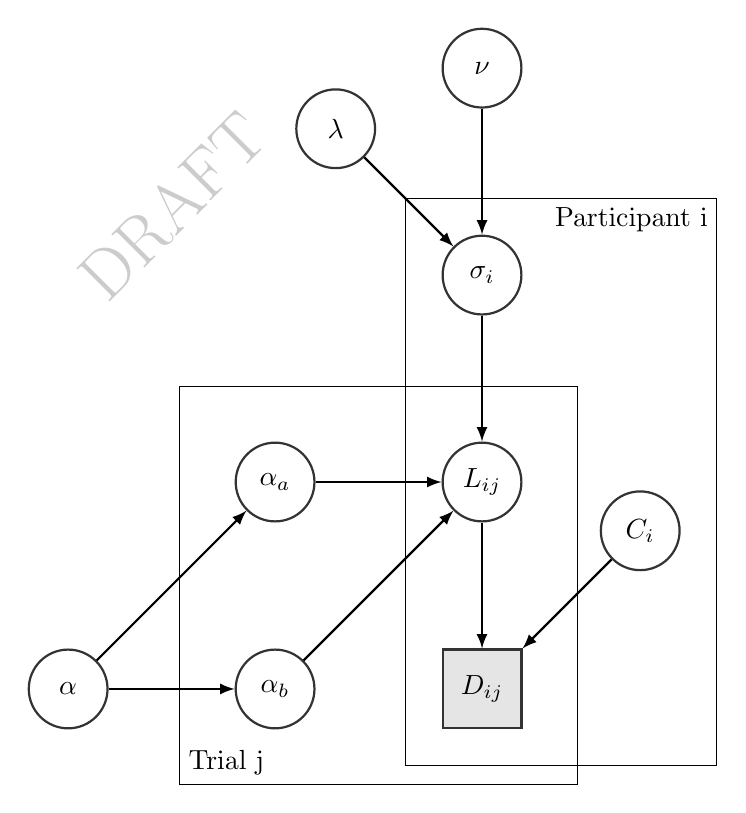
\begin{tikzpicture}
\tikzstyle{maincir}=[circle, minimum size = 10mm, thick, draw =black!80, node distance = 16mm]
\tikzstyle{mainsq}=[rectangle, minimum size = 10mm, thick, draw =black!80, node distance = 16mm]
\tikzstyle{connect}=[-latex, thick]
\tikzstyle{i} = [rectangle, draw, minimum height=26em, minimum width=50em]
\tikzstyle{box}=[rectangle, draw=black!100]

  \node[mainsq, fill = black!10] (D)  {$D_{ij}$ };
  \node[maincir] (L) [above=of D] {$L_{ij}$ };
  \node[maincir] (C) [above right=of D] {$C_{i}$ };
  \node[maincir] (S) [above=of L] {$\sigma_{i}$ };
  \node[maincir] (lambda) [above left=of S] {$\lambda$ };
  \node[maincir] (nu) [above=of S] {$\nu$};
  \node[maincir] (A) [left=of L] {$\alpha_a$ };
  \node[maincir] (AII) [below=of A] {$\alpha_b$ };
  \node[maincir] (Aparent) [left=of AII]{$\alpha$ };


  \path (L) edge [connect] (D)
        (C) edge [connect] (D)
        (S) edge [connect] (L)
        (A) edge [connect] (L)
        (AII) edge [connect] (L)
        (lambda) edge [connect] (S)
        (nu) edge [connect] (S)
        (Aparent) edge [connect] (A)
        (Aparent) edge [connect] (AII);

 \node[rectangle, inner sep=7mm, draw=black!100, fit= (L) (D) (A)](itemrect) {};
 \node[anchor=south west] at (itemrect.south west) {Trial j};
 \node[rectangle, inner sep=4.6mm, draw=black!100, fit= (L) (D) (S) (C)](ppntrect) {};
 \node[anchor=north east] at (ppntrect.north east) {Participant i};

\end{tikzpicture}
\caption{Model diagram showing the implementation of the \thurstone{} model. Variable definitions are given in Table \ref{modelnotation}. }
\label{modeldiagram}
\end{figure}

The acceptability strength scores are inferred using the following decision process mapping acceptability strength to choice responses:
When presented with test items $a$ and $b$ on trial $j$, participant $i$ samples an acceptability strength for each item. By definition, these samples come from normal distributions with means centered at the group's consensual acceptability score for each item, $\alpha_a$ and $\alpha_b$. Each participant has their own degree of variability around the shared mean, $\sigma_i$. The participant then takes the difference between the perceived acceptability scores on this trial, $L_{ij}$, and compares it to their criterion level $C_i$. The criterion determines how each participant maps their perception of the acceptability difference onto the response options. If the absolute difference is greater than the criterion value, the participant indicates the preference indicated by the sign of the difference, otherwise they indicate no preference. Although different in some respects, this mapping process follows similar motivating logic to a scheme previously described by \citet{bader2010sigdetection}
for mapping between graded sentence acceptability responses and binary ones.

\begin{table}
  \caption{Parameter descriptions}
  \label{modelnotation}
  \centering
  \begin{tabular}{lll}  %        \toprule
  Variable    & Meaning & Distributed as \\ \hline
  %$D_{ij}$ & Observed decision & \begin{equation*}D=\begin{cases} 1, &\text{if}\ L_{ij}>C_i \\ -1, &\text{if}\ L_{ij}<-C_i\\ 0,&\text{otherwise}\end{cases} \end{equation*} \\

  $D_{ij}$ & Observed decision & $1$ if $L_{ij}>C$, $-1$ if $L_{ij}< -C$, 0 otherwise \\

  $L_{ij}$ & Decision variable for trial $j$ & $N(\alpha_a-\alpha_b,\sigma_i)$ \\
  $C$ & Participant decision criterion & $U(1,50)$ \\
  $\sigma$ & Participant variability & $Weibull(\lambda,\nu)$ \\
  $\lambda$ & Variability hyperparameter & $\lvert N(2,5) \rvert$ \\
  $\nu$ & Variability hyperparameter & $\lvert N(0.02,0.04) \rvert$ \\
  $\alpha$ & Item acceptability  & $N(0,20)$ \\
  \end{tabular}
\end{table}


\section*{Acknowledgments}
All human research reported here complied with Adelaide University's ethics requirements. SL was supported through the provision of an Australian Government Research Training Program Scholarship. DN received salary support from ARC grant FT110100431, AP from ARC grants DP110104949 and DP150103280, and ATH from ARC grants DP110104949 and DE120102378.
The authors would like to thank Dr Kleanthes Grohmann for his helpful comments on this work, and Jon Sprouse for permission to make quantitative comparisons with previous research data.

\section*{Competing interests}
The authors have no competing interests to declare.

% bib
\bibliography{soc,thurstone_supp}
\bibliographystyle{apacite}

\end{document}
